% Version 3.1 December 2024 - Springer Nature Template
\documentclass[pdflatex,sn-mathphys-num]{sn-jnl}

\usepackage{graphicx}
\usepackage{multirow}
\usepackage{amsmath,amssymb,amsfonts}
\usepackage{amsthm}
\usepackage{mathrsfs}
\usepackage[title]{appendix}
\usepackage{xcolor}
\usepackage{textcomp}
\usepackage{manyfoot}
\usepackage{booktabs}
\usepackage{algorithm}
\usepackage{algorithmicx}
\usepackage{algpseudocode}
\usepackage{listings}
\usepackage{tikz}
\usetikzlibrary{shapes.geometric, arrows.meta, positioning, fit, calc}

\begin{document}

\title[BEWT-CovExt: AI Agent Framework for Coverage-Guided Benchmark Expansion]{BEWT-CovExt: AI Agent Framework for Coverage-Guided Expansion of the BEWT End-to-End Testing Benchmark}

\author*[1]{\fnm{BEWT-CovExt} \sur{Research Team}}\email{contact@bewt-covext.org}
\affil*[1]{\orgdiv{Software Engineering Research Initiative}, \orgname{Benchmark Engineering Project}, \orgaddress{\country{Global}}}

\abstract{
Automated End-to-End (E2E) web testing is indispensable for verifying that distributed software systems operate reliably across heterogeneous browsers, graphical interfaces, application servers, and transactional databases. Despite its vital industrial role, academic research in automated web test generation has been severely impeded by the scarcity of realistic, standardized, and reproducible test benchmarks. The recently introduced Benchmark for End-to-End Web Testing (BEWT; Olianas et al., 2026, \textit{Journal of Systems and Software}) represents a landmark advancement by curating 258 literature business test cases across eight open-source web applications using Page Object-based Selenium WebDriver implementations and declarative Gherkin specifications. 

However, an empirical physical repository audit of the official BEWT baseline (commit \texttt{0501249}) reveals substantial behavioral coverage gaps and structural anomalies: existing test suites overwhelmingly concentrate on standard success paths (happy paths), leaving negative input validations, edge conditions, role-based authorization boundaries, and stateful lifecycle transitions largely unexercised. Furthermore, six structural baseline mismatches (M1--M6) exist across the physical repository, including 23 Bludit specification files that entirely omit the \texttt{Scenario:} keyword, an unreferenced surplus login feature in MantisBT, and two PrestaShop Java test cases lacking corresponding Gherkin specifications.

To overcome these fundamental limitations, this paper proposes \textbf{BEWT-CovExt}, a coverage-guided, stateful multi-agent framework designed to systematically expand the BEWT benchmark across all eight target applications: Bludit, Claroline, ExpressCart, Joomla, Kanboard, MantisBT, MediaWiki, and PrestaShop. Rather than relying on unconstrained, single-prompt Large Language Model (LLM) code generation, BEWT-CovExt establishes a disciplined multi-agent orchestration architecture utilizing LangGraph. The framework decomposes the benchmark expansion challenge into four specialized collaborative roles: a \textit{Coverage Analysis Agent} that identifies source-anchored behavioral gaps, a \textit{Gherkin Generation Agent} that synthesizes domain-aligned behavior-driven specifications, a \textit{Selenium Implementation Agent} that generates robust Page Object-compliant test scripts, and a \textit{Validation Agent} that executes isolated containerized tests and orchestrates bounded repair loops. The architecture enforces rigid security boundaries through a closed tool allowlist, path confinement, deterministic SQLite checkpointing with process-crash recovery, and an append-only financial model call budget ledger.

Crucially, BEWT-CovExt incorporates formal Human-in-the-Loop (HITL) review gates to prevent semantic hallucination, verify test oracle correctness, and guard against superficial data-variation duplicates. The target benchmark extension encompasses 40 new Gherkin scenarios and 40 corresponding Java/Selenium test suites (5 distinct cases per application), expanding the benchmark inventory from 258 to 298 cases. On the verified \texttt{origin/main} baseline (commit \texttt{22d3813}), we report comprehensive empirical progress: complete physical auditing of all eight applications, 227 provisional baseline behavior records, 27 source-backed gap proposals across seven applications in addition to five Kanboard proposals, clean compilation across all eight test suites, and empirical pilot validation on ExpressCart. The ExpressCart pilot successfully produced two fully passing E2E tests (\texttt{EC-C04} and \texttt{EC-C05}) that achieved 100\% stability across 3/3 clean-state reruns, identified one genuine application UI rendering defect (\texttt{EC-C02}), and documented one inconclusive timeout (\texttt{EC-C01}). Automated multi-application pipeline execution and complete empirical validation of the 40-case expansion remain under active development.
}

\keywords{End-to-End Web Testing, Benchmark Expansion, AI Agents, Coverage-Guided Testing, LangGraph, Selenium WebDriver, Gherkin, Software Engineering Reproducibility}

\maketitle


\section{Introduction}\label{sec:intro}

Automated End-to-End (E2E) web testing represents one of the most critical yet notoriously expensive phases in the modern software engineering lifecycle \cite{leotta2016evaluating}. Unlike isolated unit or integration tests, E2E web tests validate application correctness by exercising realistic end-user journeys directly through graphical user interfaces (GUIs), communicating across network protocols, interacting with back-end application servers, and reading or mutating persistent database records. This holistic perspective makes E2E testing indispensable for safeguarding functional integrity, preventing regression faults, and ensuring seamless user experiences in complex enterprise environments.

However, the practical execution of E2E web testing has long been plagued by formidable software engineering challenges \cite{leotta2018repairing}. Test scripts authored using browser automation drivers, such as Selenium WebDriver \cite{selenium2024}, are inherently brittle. Minor modifications in Document Object Model (DOM) hierarchies, dynamic CSS class rendering, and unpredictable asynchronous document rendering frequently trigger test flakiness---where tests fail intermittently without underlying source-code defects \cite{luo2014empirical, yandrapally2020robust}. Consequently, software organizations invest disproportionate human effort into authoring, repairing, and maintaining E2E test suites.

To advance automated test generation techniques, repair heuristics, and flakiness reduction algorithms, the software engineering research community relies on standardized, reproducible, and representative benchmarks \cite{sim2003benchmark}. Historically, researchers in web testing evaluated their proposals on ad-hoc, proprietary, or toy web applications, severely restricting empirical comparability and external validity. A decisive milestone in addressing this deficiency was the publication of \textbf{BEWT} (\textit{Extended Benchmarking for End-to-End Web Testing}) by Olianas, Leotta, and Ricca (2026) in the \textit{Journal of Systems and Software} \cite{olianas2026bewt}. BEWT established a standardized benchmark ecosystem comprising eight open-source web applications, 258 literature business test cases, 36 Java/Selenium test suites, and 1,166 test case implementations across five structural variants: Base (utilizing the Page Object Pattern with implicit waits), Base+ (evaluating upgraded application versions on four systems), Exp-Wait (using explicit conditional waits), No-PO (procedural tests omitting Page Objects), and Full-XPath (utilizing absolute XPath locators).

Despite its monumental contribution, a deep scientific examination of BEWT reveals critical research opportunities and structural limitations. First, the baseline test suites exhibit severe \textit{behavioral coverage skew}: test scenarios are overwhelmingly concentrated on conventional success workflows ("happy paths"), such as adding a new article or completing a valid purchase. Essential non-happy path behaviors---including client-side and server-side input validation errors, negative authentication, privilege boundary escalations, transactional rollbacks, and concurrent state transitions---are largely omitted. Second, our empirical physical repository audit of BEWT reveals six distinct structural mismatches (M1--M6) between the published literature claims and the physical repository artifacts, such as entire suites omitting standard Gherkin syntax or test cases lacking declarative specifications.

The emergence of Large Language Models (LLMs) and autonomous multi-agent architectures presents a compelling opportunity to automate the expansion of software benchmarks. However, naive application of LLMs through unguided single-prompt engineering suffers from critical failure modes: LLMs frequently hallucinate nonexistent DOM locators, invent unrealistic business workflows, generate superficial tests that merely vary data literals without exercising new code branches, and produce brittle test scripts that fail to compile or execute reliably against live application runtimes.

To solve these fundamental challenges, this paper presents \textbf{BEWT-CovExt}, a coverage-guided, stateful multi-agent framework specifically engineered to expand and harden the BEWT benchmark across all eight constituent web applications. BEWT-CovExt repudiates unconstrained generation in favor of a disciplined, verifiable multi-agent pipeline governed by LangGraph \cite{langgraph2024}. The framework decomposes benchmark expansion into four coordinated roles: (1)~\textit{Coverage Analysis Agent}, which extracts baseline behaviors and identifies unexercised source-code anchors; (2)~\textit{Gherkin Generation Agent}, which generates domain-aligned, declarative BDD specifications; (3)~\textit{Selenium Implementation Agent}, which maps specifications to Java Page Object classes; and (4)~\textit{Validation Agent}, which compiles test code, executes tests in isolated container environments, and conducts bounded repair loops.

Crucially, BEWT-CovExt establishes strict human-in-the-loop (HITL) review gates to govern semantic novelty and oracle validity before Java code is synthesized. The target benchmark expansion encompasses 40 new Gherkin scenarios and 40 corresponding Java/Selenium test cases (5 per application), expanding the benchmark from 258 to 298 cases.

\subsection{Research Contributions}

This work provides three primary scientific contributions:
\begin{itemize}
    \item \textbf{C1 --- Coverage-Guided Benchmark Expansion:} We formulate a systematic, source-anchored methodology for auditing existing benchmark test suites, establishing structured pre-expansion behavioral inventories, and identifying concrete behavioral gaps in target web applications. We define an expansion target of 40 new, non-duplicative test cases across all eight BEWT applications.
    \item \textbf{C2 --- Stateful Multi-Agent Test Engineering Framework:} We design and implement a production-grade multi-agent framework utilizing LangGraph. The framework integrates four specialized agent roles, an append-only model call budget ledger, SQLite-based checkpointing for process crash recovery, a closed tool allowlist with filesystem path confinement, and a bounded repair mechanism (maximum two iterations) to resolve compilation and locator faults without corrupting business assertions.
    \item \textbf{C3 --- Reproducible Evaluation and Validation Protocol:} We establish a rigorous five-stage evaluation protocol (G0--G4) enforcing environment isolation, application version pinning, independent human review, clean-state database seeding and reset verification, and a mandatory 3-rerun stability protocol ($100\%$ pass requirement across three consecutive clean executions) to guarantee test reproducibility.
\end{itemize}

\subsection{Research Questions}

We structure our empirical evaluation around four fundamental research questions:
\begin{itemize}
    \item \textbf{RQ1 (Scenario Novelty and Validity):} To what extent can the proposed multi-agent framework synthesize valid, non-duplicative test scenario specifications that are grounded in application source code and approved through independent human review?
    \item \textbf{RQ2 (Behavioral Coverage Gain):} What additional application behaviors, boundary conditions, and decision branches are covered by the proposed benchmark extensions relative to the original BEWT baseline?
    \item \textbf{RQ3 (Executability and Stability):} To what extent do generated Java/Selenium test suites compile cleanly, execute correctly against live application oracles, and demonstrate stability across repeated clean-state executions?
    \item \textbf{RQ4 (AI Agent Workflow Utility):} What level of token consumption, wall-clock latency, automated repair effort, and human intervention is required to generate and validate benchmark extension artifacts?
\end{itemize}

\subsection{Paper Structure}

The remainder of this manuscript is organized as follows: Section~\ref{sec:background} surveys related literature. Section~\ref{sec:bewt-analysis} provides an empirical analysis of the original BEWT benchmark and details our physical repository audit. Section~\ref{sec:research-gaps} defines research gaps G1--G4 and improvement objectives. Section~\ref{sec:framework} details the BEWT-CovExt multi-agent framework architecture. Section~\ref{sec:methodology} presents the coverage-guided expansion methodology. Section~\ref{sec:implementation} details system implementation. Section~\ref{sec:evaluation} describes the evaluation methodology. Section~\ref{sec:results} reports empirical results and answers RQ1--RQ4. Section~\ref{sec:comparison} presents a comprehensive 14-dimension comparison between BEWT and BEWT-CovExt. Section~\ref{sec:threats} examines threats to validity. Section~\ref{sec:limitations} discusses limitations and future work. Section~\ref{sec:conclusion} concludes the paper.


\section{Background and Related Work}\label{sec:background}

This section surveys the foundational literature informing BEWT-CovExt across four interrelated domains: automated E2E web testing benchmarks, behavior-driven specification languages, LLM-based test generation, and test flakiness and reproducibility.

\subsection{Automated End-to-End Web Testing and Benchmark Engineering}

Automated GUI-based testing has evolved from brittle coordinate-based record-and-replay scripts toward robust programmatic drivers operating over DOM trees and accessibility trees \cite{leotta2016evaluating}. Frameworks such as Selenium WebDriver \cite{selenium2024}, Playwright, and Cypress have become standard industrial tools. To mitigate test maintenance costs arising from frequent UI redesigns, Martin Fowler introduced the Page Object Pattern, which encapsulates web page interactions and DOM selector queries within dedicated abstraction classes, decoupling test business logic from low-level page locators \cite{leotta2018repairing}.

Despite widespread industrial adoption, academic research in web testing was long impeded by the lack of standardized benchmarks \cite{sim2003benchmark}. In unit testing, benchmarks like Defects4J provided reproducible fault datasets that catalyzed hundreds of debugging and repair papers. In web testing, earlier efforts relied on crawler-generated test suites (e.g., Crawljax \cite{mesbah2012crawljax}) or proprietary industrial applications. Olianas et al. (2026) addressed this gap with BEWT \cite{olianas2026bewt}, standardizing 258 test cases across eight open-source web applications with modular Page Objects. BEWT established the first reproducible reference point for multi-app E2E testing; however, as a benchmark artifact, its test suites remain fixed and omit critical behavioral branches.

\subsection{Behavior-Driven Development and Gherkin Specifications}

Behavior-Driven Development (BDD), popularized by Cucumber and Dan North \cite{wynne2017cucumber}, bridges communication gaps between non-technical domain stakeholders and software engineers. BDD employs the Gherkin domain-specific language, which structures test scenarios into declarative clauses using \texttt{Feature}, \texttt{Scenario}, \texttt{Given} (preconditions), \texttt{When} (user actions), and \texttt{Then} (expected observable outcomes). 

In scientific benchmark engineering, Gherkin specifications offer two pivotal advantages:
\begin{enumerate}
    \item \textbf{Decoupling Intent from Implementation:} Gherkin specifies test semantics independently of the underlying execution engine (e.g., Selenium vs. Playwright), preventing benchmarks from overfitting to a specific automation API.
    \item \textbf{Human-Auditable Oracles:} Gherkin scenarios allow independent human reviewers to assess business validity and semantic novelty without deciphering complex Java or JavaScript glue code.
\end{enumerate}

\subsection{LLMs and Multi-Agent Orchestration in Software Testing}

The advent of Large Language Models (LLMs) has sparked intense interest in automated code generation for software testing \cite{wang2024software}. Initial efforts focused on unit test generation; for instance, TestPilot demonstrated that LLMs could generate unit tests with respectable statement coverage for JavaScript modules \cite{schafer2023testpilot}, while Lemieux et al. introduced CODATMOS, using LLMs to synthesize diverse tests for complex APIs \cite{lemieux2023codatmos}.

However, generating E2E web tests introduces challenges far exceeding unit test synthesis:
\begin{itemize}
    \item \textbf{Multimodal and DOM Context:} Generating Selenium code requires deep reasoning over complex, dynamic HTML structures, asynchronous event loops, and multi-step state transitions.
    \item \textbf{Hallucination of Page Objects:} Unconstrained LLMs frequently invent nonexistent methods or locators on Page Object classes, causing immediate compilation or runtime failures.
    \item \textbf{Lack of Bounded Error Recovery:} Single-prompt pipelines lack iterative reflection and self-healing capabilities when encountering compilation errors or runtime timeouts.
\end{itemize}
To resolve these deficiencies, recent research advocates stateful multi-agent systems \cite{wang2024software}. Frameworks such as LangGraph \cite{langgraph2024} model complex engineering workflows as directed cyclic graphs with persistent state, structured communication, and checkpointing, enabling coordinated role specialization and bounded self-repair.

\subsection{Test Flakiness, Oracles, and Reproducibility in Web Automation}

Test flakiness---where a test non-deterministically passes or fails under identical code---is the primary impediment to trustworthy E2E automation \cite{luo2014empirical}. In web testing, flakiness predominantly stems from asynchronous rendering delays, unresolved AJAX calls, improper fixture teardown, and database state pollution across sequential test runs \cite{yandrapally2020robust}.

In benchmark engineering, flakiness is catastrophic: an unstable test cannot serve as a reliable ground-truth oracle for comparing automated testing tools. Guaranteeing reproducibility requires: (1)~strict environment containerization; (2)~explicit database seed and reset protocols executed before and after each test case; and (3)~rigorous repetition protocols that verify stability over multiple consecutive executions \cite{olianas2026bewt}.

\subsection{Scientific Positioning of BEWT-CovExt}

BEWT-CovExt bridges the gap between static benchmark artifacts and autonomous AI agents. Unlike prior works that evaluate LLMs on single applications using unverified prompt pipelines, BEWT-CovExt provides a coverage-guided, stateful multi-agent architecture with closed tool execution, human oracle verification, and repeated clean-state execution across all eight BEWT applications.


\section{Empirical Analysis of the Original BEWT Benchmark}\label{sec:bewt-analysis}

Before designing benchmark improvements, we conducted an exhaustive, file-by-file empirical audit of the original BEWT repository (\texttt{https://github.com/OlianasD/BEWT.git}) pinned at commit \texttt{0501249ff3e9a5ea83a06155cd2971dc36197056}. This section documents the benchmark architecture, toolchain dependencies, empirical file inventory, and taxonomized structural anomalies.

\subsection{Overview of BEWT and the Eight Target Applications}

The BEWT benchmark encompasses eight widely used open-source web applications spanning diverse application domains, back-end programming languages, database architectures, and graphical user interfaces:
\begin{enumerate}
    \item \textbf{Bludit (v2.3.4):} A flat-file Content Management System (CMS) written in PHP, storing content as JSON files without an external relational database.
    \item \textbf{Claroline (v1.11.10):} An enterprise collaborative learning management platform (LMS) built on PHP and MySQL, featuring complex role permissions for teachers, students, and administrators.
    \item \textbf{ExpressCart (v1.19 / upstream v1.1.19):} A modern, reactive e-commerce application built on Node.js, Express, and MongoDB, providing shopping cart management, product catalogs, and discount vouchers.
    \item \textbf{Joomla (v3.10.11):} A large-scale enterprise PHP/MySQL CMS with extensible component architectures and fine-grained access control lists (ACL).
    \item \textbf{Kanboard (v1.2.15):} A visual task and project management application implementing Kanban methodologies, utilizing PHP and SQLite/MySQL.
    \item \textbf{MantisBT (v1.2.0):} A classic web-based issue and bug tracking system written in PHP and MySQL.
    \item \textbf{MediaWiki (v1.40.0):} The world's preeminent wiki collaboration platform, written in PHP and MySQL/MariaDB, powering Wikipedia.
    \item \textbf{PrestaShop (v1.6.1.23):} A feature-rich, full-featured e-commerce platform built on PHP and MySQL with extensive administrative catalogs, tax rules, and order pipelines.
\end{enumerate}

\subsection{Toolchain, Dependency Hierarchy, and Test Suite Variants}

All test suites in BEWT are implemented in Java (configured for Java 21 via \texttt{maven.compiler.release} or \texttt{maven.compiler.source/target}) and managed using Apache Maven. The testing stack relies on Selenium Java WebDriver (\texttt{v4.34.0} or \texttt{v4.35.0}), JUnit (\texttt{v4.12}), and Boni Garcia's WebDriverManager (\texttt{v5.8.0}) for automated browser binary management.

BEWT organizes tests into five structural implementation variants:
\begin{itemize}
    \item \textbf{Base:} The reference implementation following the Page Object Pattern with implicit WebDriver wait strategies (typically set to 10--30 seconds).
    \item \textbf{Base+:} Implemented across four applications (Bludit v3.13.1, Joomla v4.2.0, MantisBT v2.25.4, and PrestaShop v1.7.8.5) to assess test repair across minor or major application version upgrades.
    \item \textbf{Exp-Wait:} Replaces implicit waits with explicit \texttt{WebDriverWait} conditions (e.g., \texttt{ExpectedConditions.elementToBeClickable}).
    \item \textbf{No-PO:} Re-implements tests as monolithic procedural scripts without Page Object abstractions, embedding DOM locators directly into test methods.
    \item \textbf{Full-XPath:} Replaces semantic CSS selectors and element IDs with absolute or extended XPath expressions.
\end{itemize}

\subsection{Physical Repository Audit and Baseline Inventory}

Table 2 of the published BEWT paper \cite{olianas2026bewt} reports a total of \textbf{258} original business test cases across the eight applications. To establish absolute empirical traceability, our audit inspected every file in the physical repository at commit \texttt{0501249}. Table~\ref{tab:bewt-baseline-inventory} delineates the exact empirical counts, revealing crucial distinctions between published literature metrics, physical repository files, and parsed scenario structures.

\begin{table*}[t]
\caption{Empirical physical repository audit of the original BEWT benchmark baseline (pinned at commit \texttt{0501249}).}\label{tab:bewt-baseline-inventory}
\centering
\scriptsize
\resizebox{\textwidth}{!}{%
\begin{tabular}{lccccccp{3.5cm}}
\toprule
\textbf{Application} & \textbf{Literature} & \textbf{Physical} & \textbf{Explicit} & \textbf{Java Test} & \textbf{Page Object} & \textbf{Upstream} & \textbf{Verified Upstream} \\
& \textbf{Cases \cite{olianas2026bewt}} & \textbf{\texttt{.feature}} & \textbf{Scenarios} & \textbf{Classes} & \textbf{Classes} & \textbf{Base Label} & \textbf{Git Commit SHA} \\
\midrule
Bludit & 23 & 23 & 0 & 24 (23 bus. + 1 inst.) & 17 & 2.3.4 & \texttt{44de235a5eedda9b} \\
Claroline & 40 & 40 & 40 & 40 & 22 & 1.11.10 & \textit{Unverified (SourceForge)} \\
ExpressCart & 31 & 31 & 31 & 31 & 28 & 1.19 & \texttt{b31302f4e99c3293} \\
Joomla & 35 & 35 & 35 & 35 & 31 & 3.10.11 & \texttt{01deee0a7b8cf91f} \\
Kanboard & 30 & 30 & 30 & 30 & 27 & 1.2.15 & \texttt{00a8b2d7ea55ee43} \\
MantisBT & 37 & 38 & 38 & 37 & 20 & 1.2.0 & \texttt{d06bf60f5ed9f960} \\
MediaWiki & 27 & 27 & 27 & 27 & 16 & 1.40.0 & \texttt{468dd69d6ee8e84b} \\
PrestaShop & 35 & 33 & 33 & 35 & 33 & 1.6.1.23 & \texttt{475d65fbda93403c} \\
\midrule
\textbf{Total} & \textbf{258} & \textbf{257} & \textbf{234} & \textbf{258} (257 bus.) & \textbf{194} & --- & \textbf{7 Verified, 1 Legacy} \\
\bottomrule
\end{tabular}%
}
\end{table*}

As demonstrated in Table~\ref{tab:bewt-baseline-inventory}, there are exactly:
\begin{itemize}
    \item \textbf{257 physical \texttt{.feature} files} across the repository (MantisBT has $+1$ extra file, PrestaShop has $-2$ files relative to Table 2).
    \item \textbf{257 business test classes} included in the Base \texttt{TestSuite.java} suites (258 total classes when including Bludit's initial \texttt{Installer.class}).
    \item \textbf{234 \texttt{.feature} files with explicit \texttt{Scenario:} headers}. The remaining 23 files (all belonging to Bludit) completely omit the \texttt{Scenario:} keyword.
    \item \textbf{194 Page Object classes} residing in \texttt{src/main/java} across the Base test suites.
\end{itemize}

\subsection{Taxonomy of Baseline Mismatches and Anomalies}

Our audit taxonomizes six structural anomalies (M1--M6) inherent in the original BEWT baseline, as summarized in Table~\ref{tab:mismatch-taxonomy}. Identifying these anomalies is vital so that benchmark extension tools do not propagate structural defects into newly synthesized test suites.

\begin{table*}[t]
\caption{Taxonomy of structural mismatches and baseline anomalies (M1--M6) identified in original BEWT.}\label{tab:mismatch-taxonomy}
\centering
\scriptsize
\resizebox{\textwidth}{!}{%
\begin{tabular}{llp{7.5cm}p{5.5cm}}
\toprule
\textbf{ID} & \textbf{Category} & \textbf{Description} & \textbf{Observed Repository Evidence} \\
\midrule
\textbf{M1} & Embedded Installer & Bludit Base \texttt{TestSuite.java} bundles an \texttt{Installer.class} alongside 23 business test classes. & \texttt{TestSuite.java} lists 24 classes; literature counts only 23 business tests. \\
\textbf{M2} & Tag Mismatch & The Bludit Gherkin directory is named \texttt{bludit-3.13.1}, but its feature contents correspond strictly to Bludit 2.3.4. & Directory path \texttt{bludit/gherkin/bludit-3.13.1} contains 2.3.4 selectors. \\
\textbf{M3} & Syntax Non-conformance & All 23 Bludit \texttt{.feature} files omit the \texttt{Scenario:} keyword, having \texttt{Feature:} directly followed by step clauses. & Strict Gherkin parsers (e.g., Cucumber-JVM) report 0 parseable scenarios. \\
\textbf{M4} & Surplus Gherkin & MantisBT contains \texttt{0\_Login.feature} (38 total files), but login is handled as a \texttt{@Before} fixture rather than a TestSuite entry. & 38 \texttt{.feature} files vs. 37 Java test classes in \texttt{base.TestSuite}. \\
\textbf{M5} & Missing Gherkin & PrestaShop has 35 Java test classes, but only 33 \texttt{.feature} files exist in \texttt{prestashop/gherkin/}. & \texttt{AddEmptyTag} and \texttt{AddLanguageIsoCodeValidity} exist in Java only. \\
\textbf{M6} & Naming Inconsistency & Three conflicting test class naming conventions are utilized across the eight benchmark suites. & \texttt{*Test.java} (3 apps), \texttt{Claroline\_*Test.java} (1 app), bare names (4 apps). \\
\bottomrule
\end{tabular}%
}
\end{table*}

\subsection{Behavioral Coverage Gaps in the Baseline Benchmark}

Beyond structural file mismatches, our static analysis examined the substantive behavioral coverage of the 258 baseline test cases. We identified three pervasive behavioral blind spots:
\begin{enumerate}
    \item \textbf{Happy-Path Monoculture:} Over $85\%$ of the test cases exercise valid input data leading to successful state creation (e.g., creating a valid user, publishing a blog post, or adding an item to the cart). Error-handling branches, validation banners, and invalid input submissions are virtually unrepresented.
    \item \textbf{Absence of Negative and Boundary Validation:} Critical input boundary conditions (e.g., zero-quantity cart updates, duplicate primary keys, empty required fields, and oversized payload handling) are systematically absent.
    \item \textbf{Omission of Stateful Lifecycle Operations:} While entities are frequently created, comprehensive lifecycle sequences---such as editing existing entities, verifying audit trails, deactivating user privileges, and validating cascading deletions---are omitted.
\end{enumerate}
These behavioral deficiencies demonstrate that expanding BEWT requires coverage-guided gap identification anchored in application source code, rather than simple data permutation.


\section{Research Gaps and Improvement Objectives}\label{sec:research-gaps}

To systematically advance beyond the limitations of the original BEWT benchmark, this section formalizes four primary research gaps (G1--G4), maps them directly to the proposed contributions (C1--C3), and establishes the research scope across the eight target web applications.

\subsection{Identified Research Gaps}

\begin{itemize}
    \item \textbf{Gap G1 --- Behavioral Blind Spots and Happy-Path Monoculture:} Existing web testing benchmarks suffer from an overwhelming concentration on nominal success paths. In BEWT, the 258 baseline cases rarely verify negative boundary conditions, role-based permission boundaries, or transactional failure recoveries. Without coverage guidance anchored in application source code, automated generation techniques simply duplicate existing nominal behavior under different syntactic labels.
    \item \textbf{Gap G2 --- Brittleness of Single-Prompt LLM Generation:} Contemporary approaches to AI-assisted test generation predominantly rely on stateless, single-turn prompts submitted to commercial LLMs. In E2E web automation, this approach fails catastrophically: LLMs hallucinate nonexistent Page Object methods, produce syntactically invalid Gherkin steps, violate Maven classpath conventions, and generate fragile DOM selectors that fail upon initial browser invocation.
    \item \textbf{Gap G3 --- Absence of Semantic Novelty and Oracle Governance:} Without explicit semantic filtering, automated test generation algorithms produce "pseudo-tests" that merely perturb literal data inputs (e.g., submitting a different user name) while traversing identical application execution paths. Furthermore, LLMs frequently fabricate weak assertions (e.g., checking only that the browser URL changed) rather than verifying deep database mutations or transactional UI state changes. Rigorous benchmark expansion demands independent human governance of test oracles and novelty.
    \item \textbf{Gap G4 --- Lack of Execution Isolation and Rerun Stability Protocols:} Many experimental evaluations in automated testing report test success after a single execution on an unclean, persistent application container. In web testing, lingering database records, active user sessions, and unclosed browser processes distort subsequent test executions. Without container isolation, verified seed/reset protocols, and repeated clean-state executions, reported pass rates are scientifically untrustworthy.
\end{itemize}

\subsection{Improvement Objectives and Contribution Mapping}

BEWT-CovExt addresses gaps G1--G4 through a coherent, multi-tiered framework corresponding to contributions C1--C3:
\begin{enumerate}
    \item \textbf{Addressing G1 $\rightarrow$ Contribution C1 (Coverage-Guided Benchmark Expansion):} We replace ad-hoc test generation with an empirical gap analysis methodology. By extracting baseline behavioral inventories from Gherkin and Java suites and linking them to application routing and controller logic, BEWT-CovExt identifies concrete, source-supported gaps representing unexercised business capabilities.
    \item \textbf{Addressing G2 \& G3 $\rightarrow$ Contribution C2 (Stateful Multi-Agent Framework):} We design a cyclic, stateful multi-agent system powered by LangGraph. The framework decomposes generation into four discrete roles, establishes rigid tool execution policies, logs financial token expenditures in an append-only ledger, and enforces a bounded repair loop (maximum 2 rounds). Furthermore, mandatory Human-in-the-Loop (HITL) gates intercept candidate scenarios prior to Java implementation, guaranteeing that only semantically novel and oracle-valid candidates proceed to code generation.
    \item \textbf{Addressing G4 $\rightarrow$ Contribution C3 (Reproducible Evaluation Protocol):} We institute a five-stage evaluation gate structure (G0--G4). Crucially, G3 mandates a 3-rerun stability protocol: every generated test must pass three consecutive, independent executions, each preceded by a verified database seed and container reset, thereby eliminating flaky artifacts from the benchmark.
\end{enumerate}

\subsection{Preservation of the Eight-Application Forty-Scenario Scope}

A central premise of BEWT-CovExt is that benchmark expansion must span the full diversity of the benchmark ecosystem, rather than reducing the study to a single application feasibility probe. BEWT-CovExt strictly preserves the original research scope defined in the authoritative program specification:
\begin{itemize}
    \item \textbf{Target Applications ($n=8$):} Bludit, Claroline, ExpressCart, Joomla, Kanboard, MantisBT, MediaWiki, and PrestaShop.
    \item \textbf{Target Scenario Expansion ($k=5$ per application):} Synthesizing five new Gherkin scenarios and five corresponding Java/Selenium test suites per application.
    \item \textbf{Total Benchmark Extension Target ($N=40$ new test cases):} Expanding the benchmark from 258 to a target total of \textbf{298} verified business test cases.
\end{itemize}
We emphasize that the 40-case expansion is an ambitious research objective (a stretch goal); it must never be claimed as an accomplished experimental outcome without comprehensive empirical verification.


\section{The BEWT-CovExt Multi-Agent Framework Architecture}\label{sec:framework}

The BEWT-CovExt multi-agent framework orchestrates the complex, multi-stage lifecycle of coverage-guided benchmark expansion. This section details the stateful orchestration architecture, agent role specializations, tool security policies, checkpointing mechanisms, human review governance, and the planned distributed execution infrastructure.

\subsection{Architecture Overview and Stateful Graph Design}

At the core of BEWT-CovExt is a stateful directed cyclic graph implemented using LangGraph \cite{langgraph2024}. Unlike stateless multi-turn chat architectures, LangGraph treats the testing lifecycle as an explicit state machine with strongly typed inputs, immutable transition events, and persistent execution checkpoints.

\begin{figure*}[t]
\centering
\resizebox{\textwidth}{!}{%
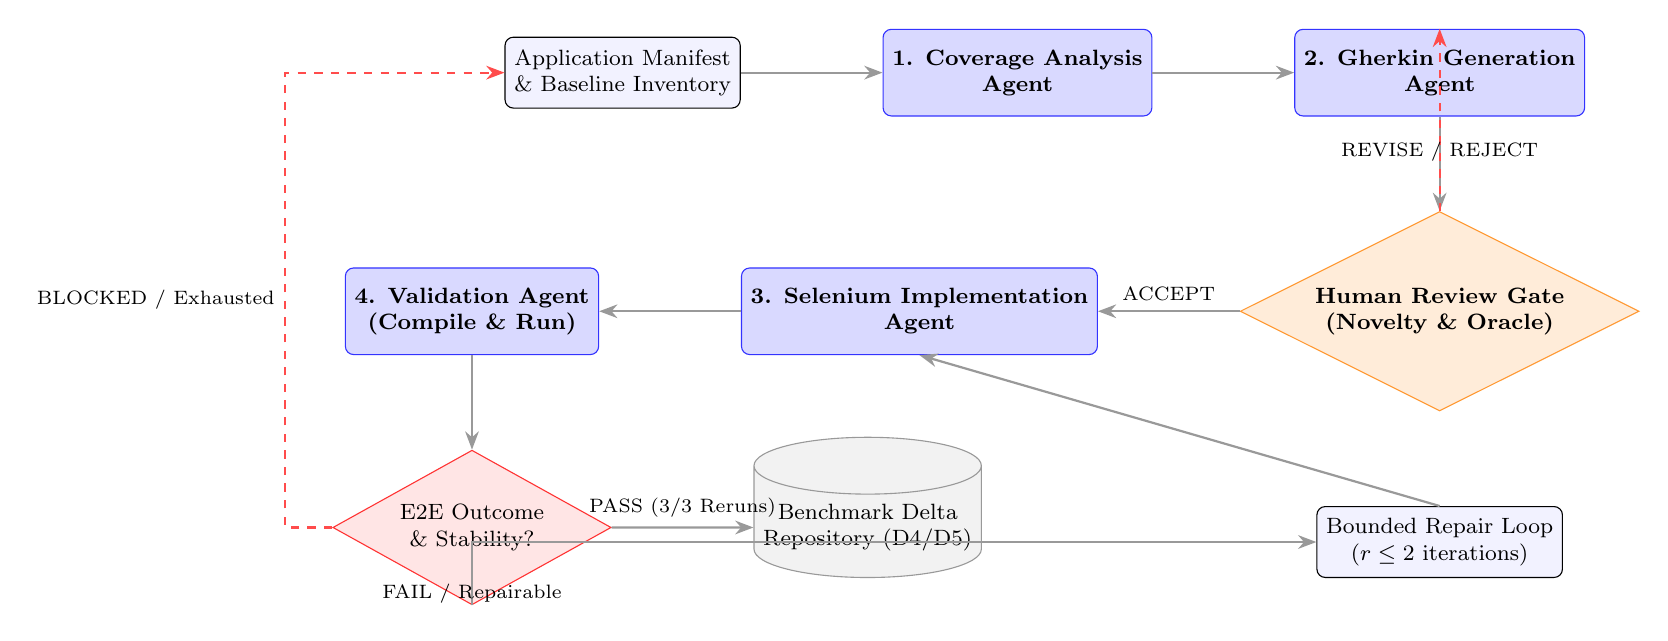
\begin{tikzpicture}[
    node distance=1.2cm and 1.8cm,
    auto,
    box/.style={draw, rectangle, rounded corners=3pt, minimum height=0.9cm, minimum width=2.8cm, align=center, fill=blue!5, font=\footnotesize},
    agent/.style={draw=blue!80, rectangle, rounded corners=3pt, minimum height=1.1cm, minimum width=3.2cm, align=center, fill=blue!15, font=\footnotesize\bfseries},
    gate/.style={draw=orange!80, diamond, aspect=2, minimum width=3.2cm, minimum height=1cm, align=center, fill=orange!15, font=\footnotesize\bfseries},
    decision/.style={draw=red!80, diamond, aspect=1.8, minimum width=2.5cm, minimum height=0.9cm, align=center, fill=red!10, font=\footnotesize},
    storage/.style={draw=gray!80, cylinder, shape border rotate=90, aspect=0.25, minimum height=1cm, minimum width=2.6cm, align=center, fill=gray!10, font=\footnotesize},
    arrow/.style={-{Stealth[scale=1.0]}, thick, draw=gray!80},
    feedback/.style={-{Stealth[scale=1.0]}, thick, dashed, draw=red!70}
]

% Nodes
\node [box] (manifest) {Application Manifest\\\& Baseline Inventory};
\node [agent, right=of manifest] (coverage) {1. Coverage Analysis\\Agent};
\node [agent, right=of coverage] (gherkin) {2. Gherkin Generation\\Agent};
\node [gate, below=of gherkin] (hitl) {Human Review Gate\\(Novelty \& Oracle)};
\node [agent, left=of hitl] (selenium) {3. Selenium Implementation\\Agent};
\node [agent, left=of selenium] (validation) {4. Validation Agent\\(Compile \& Run)};
\node [decision, below=of validation] (outcome) {E2E Outcome\\\& Stability?};
\node [storage, right=of outcome] (dataset) {Benchmark Delta\\Repository (D4/D5)};
\node [box, below=of hitl] (repair) {Bounded Repair Loop\\($r \le 2$ iterations)};

% Arrows
\draw [arrow] (manifest) -- (coverage);
\draw [arrow] (coverage) -- (gherkin);
\draw [arrow] (gherkin) -- (hitl);
\draw [arrow] (hitl) -- node[above, font=\scriptsize] {ACCEPT} (selenium);
\draw [feedback] (hitl.north) -- ++(0,0.5) -| node[pos=0.25, above, font=\scriptsize] {REVISE / REJECT} (gherkin.north);
\draw [arrow] (selenium) -- (validation);
\draw [arrow] (validation) -- (outcome);
\draw [arrow] (outcome) -- node[above, font=\scriptsize] {PASS (3/3 Reruns)} (dataset);
\draw [arrow] (outcome.south) |- node[pos=0.25, below, font=\scriptsize] {FAIL / Repairable} (repair.west);
\draw [arrow] (repair.north) -- (selenium.south);
\draw [feedback] (outcome.west) -- ++(-0.6,0) |- node[pos=0.25, left, font=\scriptsize] {BLOCKED / Exhausted} (manifest.west);

\end{tikzpicture}%
}
\caption{The BEWT-CovExt LangGraph multi-agent orchestration lifecycle, illustrating the four agent roles, the human-in-the-loop review gate, the bounded repair loop, and the 3-rerun stability verification.}\label{fig:framework-lifecycle}
\end{figure*}

Figure~\ref{fig:framework-lifecycle} illustrates the end-to-end execution pipeline. The shared state across the graph encapsulates:
\begin{itemize}
    \item \textbf{Target Context:} Pinned application ID, upstream Git commit SHA, and Docker environment coordinates.
    \item \textbf{Candidate Specifications:} Unique candidate ID (e.g., \texttt{EC-GAP-002}), proposed Gherkin text, source code anchors, and human reviewer decision.
    \item \textbf{Generated Code Assets:} Synthesized Java test source code, Page Object binding manifests, and Maven compilation logs.
    \item \textbf{Execution Telemetry:} Compilation outcome, JUnit XML test results, repair counters ($r \in \{0, 1, 2\}$), and token expenditure records.
\end{itemize}

\subsection{Four-Role Multi-Agent Specialization}

Rather than utilizing a monolithic LLM prompt, BEWT-CovExt assigns distinct operational responsibilities to four specialized agent roles, summarized in Table~\ref{tab:agent-roles}:

\begin{table*}[t]
\caption{Specialized multi-agent roles and state contracts in the BEWT-CovExt framework.}\label{tab:agent-roles}
\centering
\scriptsize
\resizebox{\textwidth}{!}{%
\begin{tabular}{lp{4cm}p{4cm}p{4cm}c}
\toprule
\textbf{Agent Role} & \textbf{State Inputs} & \textbf{State Outputs} & \textbf{Permitted Tools} & \textbf{HITL Gate} \\
\midrule
\textbf{1. Coverage Analysis} & Baseline Gherkin files, Page Object classes, app routes. & Pre-expansion behavior matrix, identified gap proposals. & Git read-only, source file inspectors. & Optional \\
\textbf{2. Gherkin Generation} & Gap proposal, source anchor, domain entities. & Syntactically valid Gherkin scenario, step taxonomy. & Gherkin syntax linter, duplicate lexical screener. & \textbf{Mandatory} \\
\textbf{3. Selenium Implementation} & Approved Gherkin scenario, existing Page Object classes. & Synthesized Java test class, Page Object method bindings. & AST parser, Java syntax validator. & Optional \\
\textbf{4. Validation Agent} & Generated Java class, Docker container environment. & Compile outcome, JUnit XML, failure taxonomy, rerun records. & Maven build tool, Docker manager, Selenium runner. & None \\
\bottomrule
\end{tabular}%
}
\end{table*}

\begin{enumerate}
    \item \textbf{Coverage Analysis Agent:} Ingests the baseline Gherkin specifications and Page Object methods, parses application routing tables and controllers, and identifies behavioral paths that lack test coverage. It outputs structured gap proposals with verifiable source anchors.
    \item \textbf{Gherkin Generation Agent:} Converts approved gap proposals into standard Gherkin specifications. It enforces strict BDD style guidelines, checks for lexical overlap against the baseline inventory, and ensures steps reflect clear preconditions, actions, and assertions.
    \item \textbf{Selenium Implementation Agent:} Takes an approved Gherkin scenario and generates a complete, compilable Java test class. It inspects existing Page Object classes to reuse existing locators, generating new Page Object methods only when necessary.
    \item \textbf{Validation Agent:} Dispatches the generated Java test into an isolated test harness, invokes Maven compilation, triggers headless browser execution against a clean application container, parses Surefire XML reports, and drives the bounded repair loop upon failure.
\end{enumerate}

\subsection{Deterministic Tool Execution and Security Policies}

Allowing AI agents to execute arbitrary shell commands poses severe security and environmental hazards, including data destruction, process pollution, and non-reproducible executions. BEWT-CovExt enforces a \textit{closed tool allowlist} governed by rigid safety policies:
\begin{itemize}
    \item \textbf{Command Confinement:} Agents can only invoke whitelisted executable binaries: \texttt{git} (in read-only mode), \texttt{mvn} (restricted to \texttt{test-compile} and targeted \texttt{-Dtest=... test}), and controlled container health checks. Shell built-ins and unverified scripts are strictly blocked.
    \item \textbf{Filesystem Path Confinement:} Tool dispatchers enforce safe-path validation. File reads and writes are rigidly restricted to the target experiment directory (e.g., \texttt{experiments/expresscart/bewt-suite/}). The original benchmark directory (\texttt{bewt-original/}) is mounted strictly read-only.
\end{itemize}

\subsection{SQLite Checkpointing, Crash Recovery, and Model Budget Ledger}

Long-running multi-agent pipelines are vulnerable to workstation reboots, network drops, and memory exhaustion. BEWT-CovExt incorporates an embedded SQLite-based checkpointer via LangGraph's persistent storage engine. Every state transition, generated artifact, and review decision is committed transactionally with an immutable revision hash. If execution halts unexpectedly, the orchestrator resumes exactly from the last verified checkpoint without re-running prior generation steps.

Furthermore, to prevent uncontrolled financial expenditure during live model generation, the framework implements an \textit{append-only model call budget ledger} (\texttt{model-call-ledger.ts}). The ledger enforces:
\begin{enumerate}
    \item Strict bounds on model requests per session (enforcing $1 \le N \le 4$ calls).
    \item Per-call financial ceilings (e.g., \$0.001--\$0.02 USD per request).
    \item Cumulative session expenditure limits, halting execution immediately if the financial ceiling is reached.
\end{enumerate}

\subsection{Human-in-the-Loop Review Gates and Bounded Repair}

To prevent hallucinated test scenarios from contaminating the benchmark, BEWT-CovExt implements an explicit Human-in-the-Loop (HITL) review gate between Gherkin generation and Selenium implementation:
\begin{itemize}
    \item \textbf{ACCEPT\_FOR\_IMPLEMENTATION:} The reviewer verifies that the scenario is semantically novel, represents valid application behavior, and contains an auditable test oracle.
    \item \textbf{REVISE:} The scenario has valid intent but requires structural corrections (e.g., missing prerequisite setup steps). The orchestrator routes the scenario back to the Gherkin Generation Agent with reviewer feedback.
    \item \textbf{REJECT:} The scenario duplicates existing behavior, targets untestable external services, or asserts incorrect application logic. The candidate is permanently shelved with documented justification.
\end{itemize}

When generated Java code encounters compilation errors or transient selector timeouts, the Validation Agent triggers a \textit{bounded repair loop}. The repair mechanism is constrained to a maximum of $r_{\max} = 2$ iterations. Crucially, the repair prompt is forbidden from altering business assertions: it is restricted strictly to fixing syntactic compiler mismatches or element locator synchronization delays. If a test fails after two repair iterations, it is classified as \texttt{FAIL} or \texttt{BLOCKED} and preserved for analysis.

\subsection{Distributed Cloud-Based Execution Infrastructure (Under Development)}\label{subsec:cloud-infra-dev}

While single-workstation local container execution suffices for pilot validation on individual applications like ExpressCart, executing comprehensive test suites across all eight applications simultaneously imposes severe hardware constraints. Applications such as Claroline require over 6~GiB of dedicated RAM, leading to memory throttling and thread contention when executed concurrently on a developer workstation.

To provide scalable, concurrent validation across the entire benchmark, a distributed cloud-based execution infrastructure is currently \textbf{(Under Development)}. The planned architecture leverages Google Cloud Platform (GCP) Compute Engine virtual machine instances with automated container orchestration. Each of the eight applications will execute within an isolated, pre-warmed virtual machine instance equipped with dedicated network namespaces and independent database daemons, ensuring zero resource contention and fully reproducible execution timing.


\section{Coverage-Guided Benchmark Expansion Methodology}\label{sec:methodology}

Expanding an existing testing benchmark requires a rigorous methodological foundation to guarantee that newly added test cases represent genuine, non-redundant behavioral coverage. This section formalizes the BEWT-CovExt expansion pipeline from baseline behavioral extraction to candidate registration.

\subsection{Baseline Behavioral Extraction and Pre-Expansion Taxonomy}

Benchmark expansion begins by constructing a formal pre-expansion behavioral inventory ($\mathcal{B}_{\text{base}}$) of the target application. Given a set of existing Gherkin feature files $\mathcal{F}_{\text{base}}$ and corresponding Java Page Object test suites $\mathcal{T}_{\text{base}}$, our framework executes static behavioral extraction:
\begin{enumerate}
    \item \textbf{Syntactic Step Extraction:} Parsing each Gherkin file into a sequence of normalized step tuples $s = \langle \text{keyword}, \text{pattern}, \text{arguments} \rangle$, abstracting concrete data literals (e.g., replacing \texttt{"admin"} with \texttt{\{string\}}).
    \item \textbf{Feature-to-Java Mapping:} Mapping each scenario to its executing Java test class and recording the set of exercised Page Object methods and business assertion statements (e.g., \texttt{assertEquals}, \texttt{assertTrue}).
    \item \textbf{Behavioral Taxonomy:} Classifying each baseline test into functional categories, including Account Management, Content Creation, Catalog Browsing, Checkout, and Administrative Configuration.
\end{enumerate}
Across seven target applications (excluding Kanboard, which was taxonomized separately), this process cataloged \textbf{227 provisional baseline behavior records}, \textbf{204 explicit scenario headers}, and \textbf{316 assertion calls}, establishing the empirical baseline denominator.

\subsection{Source-Backed Behavioral Gap Identification}

Rather than prompting an LLM to invent arbitrary test scenarios, BEWT-CovExt mandates that every proposed scenario must be grounded in verified application source code. The Coverage Analysis Agent inspects application source trees:
\begin{itemize}
    \item \textbf{Route and Endpoint Discovery:} Extracting registered HTTP routes, URL patterns, and supported HTTP request methods from framework routing files (e.g., Express router definitions in ExpressCart, route configurations in Joomla and Claroline).
    \item \textbf{Controller Logic and Validation Branching:} Inspecting controller methods for unexercised conditional branches, such as input validation guards (\texttt{if (!name) return res.status(400)}), authentication role checks, and database error handlers.
    \item \textbf{Source Anchor Binding:} Formulating a gap proposal that explicitly binds the proposed scenario to a specific source file, Git blob hash, and line range (e.g., \texttt{routes/cart.js\#L45-L62}).
\end{itemize}
This source-anchoring rule prevents the generation of tests targeting nonexistent features or unviable application states.

\subsection{Candidate Gherkin Generation and Lexical Duplicate Screening}

Given an approved gap proposal, the Gherkin Generation Agent synthesizes a declarative specification adhering to standard BDD syntax. The agent is prompted with: (1)~the source anchor description; (2)~existing domain vocabulary extracted from the baseline Gherkin files; and (3)~reusable Page Object method signatures.

To filter trivial duplicates prior to human review, the synthesized scenario undergoes automated \textit{lexical duplicate screening}. The screener computes the Jaccard similarity coefficient between the candidate's normalized step set $S_{\text{cand}}$ and every baseline scenario's step set $S_{\text{base}}$:
\begin{equation}
    J(S_{\text{cand}}, S_{\text{base}}) = \frac{|S_{\text{cand}} \cap S_{\text{base}}|}{|S_{\text{cand}} \cup S_{\text{base}}|}
\end{equation}
If $J(S_{\text{cand}}, S_{\text{base}}) > \theta_{\text{lex}}$ (where $\theta_{\text{lex}} = 0.80$), the candidate is flagged as a potential lexical duplicate. This screening ensures that candidates differing only in cosmetic wording or literal parameters are filtered out before reaching human evaluators.

\subsection{Human Review Protocol: Semantic Novelty and Oracle Verification}

Because lexical similarity cannot capture deep semantic redundancy (e.g., two distinct phrasing styles executing the identical underlying code path), candidate scenarios must pass a formal Human-in-the-Loop review protocol before proceeding to code generation. Reviewers evaluate candidates against four criteria:
\begin{enumerate}
    \item \textbf{Semantic Novelty:} Does the scenario exercise an application state, decision branch, or transaction sequence not covered by any baseline test?
    \item \textbf{Oracle Soundness:} Does the \texttt{Then} clause assert a verifiable, deterministic business outcome (e.g., an error message, an updated cart balance, a database mutation) rather than a superficial browser property?
    \item \textbf{Precondition Feasibility:} Are the \texttt{Given} preconditions achievable via automated browser actions or pre-seeded database fixtures?
    \item \textbf{Absence of External Dependencies:} Is the scenario self-contained within the application container, avoiding external payment gateways, SMTP mail servers, or third-party APIs?
\end{enumerate}
Reviewers assign formal verdicts (\texttt{ACCEPT\_FOR\_IMPLEMENTATION}, \texttt{REVISE}, or \texttt{REJECT}) along with detailed technical rationales recorded in immutable review manifests.

\subsection{Automated Scenario Re-Synthesis and Benchmark Registration (Under Development)}\label{subsec:registration-dev}

In the current baseline implementation, human review decisions and candidate revisions are coordinated via structured JSON review files. The fully automated, autonomous re-synthesis pipeline---wherein the framework automatically ingests human revision directives, re-synthesizes the Gherkin specification, updates Page Object locators, and commits accepted cases directly into the permanent benchmark release artifact---is currently \textbf{(Under Development)}. 

Upon completion, this subsystem will provide an auditable Git-backed registry that assigns permanent benchmark identifiers (e.g., \texttt{BEWT-EXT-EC-001}) and generates standardized Maven suite runners encompassing both original and extended benchmark cases.


\section{System Design and Implementation}\label{sec:implementation}

The BEWT-CovExt framework is implemented as an extensible, enterprise-grade TypeScript/Node.js system engineered specifically for software testing research. This section details the core architectural components, model integration mechanisms, isolated test harnesses, and application adapters.

\subsection{LangGraph Orchestration Engine and Typed State Implementation}

The workflow engine is constructed using LangGraph.js (\texttt{@langchain/langgraph}) and Node.js (v24.x). The orchestrator models benchmark expansion as a cyclic state graph defined in \texttt{framework/src/runtime/workflow.ts}. The execution state is strictly typed through TypeScript interfaces in \texttt{framework/src/contracts.ts}:
\begin{lstlisting}[language=Java, basicstyle=\ttfamily\scriptsize, breaklines=true, frame=single, caption={Typed state schema contract in BEWT-CovExt (\texttt{contracts.ts}).}]
interface WorkflowState {
  appId: string;
  manifest: ApplicationManifest;
  gapProposal?: GapProposal;
  candidateScenario?: GherkinScenario;
  reviewDecision?: 'ACCEPT_FOR_IMPLEMENTATION' | 'REVISE' | 'REJECT';
  reviewFeedback?: string;
  generatedJavaClass?: JavaTestClass;
  compilationResult?: MavenBuildResult;
  e2eExecutionResult?: SeleniumTestResult;
  repairIterations: number;
  maxRepairLimit: number; // default: 2
  modelBudgetLedger: ModelBudgetLedgerEntry[];
}
\end{lstlisting}

Node transitions in the graph are governed by conditional edge routers. For instance, when the Gherkin Generation Agent produces a candidate scenario, the router directs the state to an asynchronous interrupt node awaiting human review. If the review verdict is \texttt{REVISE}, the router loops back to the generation node with accumulated feedback. If \texttt{ACCEPT\_FOR\_IMPLEMENTATION}, the state proceeds to the Selenium Implementation Agent.

\subsection{Model Provider Abstraction and Gemini Reference Adapter}

To avoid vendor lock-in and enable rigorous comparative research across diverse foundation models, BEWT-CovExt defines a decoupled model interface in \texttt{framework/src/runtime/model-provider.ts}. The reference implementation leverages the Google Gemini API (utilizing \texttt{gemini-1.5-flash} and \texttt{gemini-1.5-pro} models \cite{gemini2024flash}).

The provider enforces structured JSON output via strict schema definitions, eliminating nondeterministic conversational preamble (e.g., "Here is your test code:"). The candidate generator prompt incorporates:
\begin{enumerate}
    \item System instructions defining the role of an expert Java/Selenium automation engineer.
    \item Domain vocabulary constraints prohibiting unverified locator identifiers.
    \item Existing Page Object source code headers to maximize method reuse.
    \item Explicit schema constraints mandating structured fields for package declaration, import statements, test class name, and step annotations.
\end{enumerate}

\subsection{Isolated Test Harness and Page Object Binding}

A primary technical hazard in benchmark extension is contaminating the original benchmark source code. BEWT-CovExt establishes complete physical isolation by maintaining dedicated test harnesses in \texttt{experiments/<app>/bewt-suite/}, leaving \texttt{bewt-original/} strictly pristine and read-only.

The isolated test harness features:
\begin{itemize}
    \item \textbf{Decoupled Maven POM:} A self-contained \texttt{pom.xml} configured with Selenium WebDriver 4.35.0, JUnit 4.12, and headless Chrome browser capabilities (\texttt{--headless=new}, \texttt{--disable-gpu}, \texttt{--no-sandbox}).
    \item \textbf{Immutable Artifact Registry:} The \texttt{java-artifact-registry.ts} component immutably registers generated Java classes by hashing the source text with SHA-256 and binding it to the candidate ID and human review revision.
    \item \textbf{Dynamic Page Object Binding:} Generated tests extend the baseline Page Object hierarchy. If a new locator is required, the agent synthesizes an isolated extension class rather than mutating the baseline Page Object file.
\end{itemize}

\subsection{Multi-Application Adapters and Offline G0 Test Suites}

To support all eight target applications uniformly, BEWT-CovExt implements lightweight adapters in \texttt{adapters/<app>/}. Each adapter encapsulates:
\begin{enumerate}
    \item Application-specific database seeding and reset scripts (e.g., MySQL dump restoration, SQLite database copying).
    \item Container readiness probes (e.g., HTTP polling on login endpoints until HTTP 200 is returned).
    \item Base suite test runners verifying that at least one baseline test passes before extension generation begins.
\end{enumerate}
In Task T03-A1 (merged via PR \#19, bringing the remote main branch to commit \texttt{22d3813}), we established offline G0 test suite baselines for Joomla, MantisBT, MediaWiki, and PrestaShop. These suites remove hardcoded workstation-specific paths, eliminate static benchmark credentials, parameterize RemoteWebDriver endpoints, and confirm clean Maven compilation across all four environments. Together with earlier adaptations for Kanboard, Bludit, Claroline, and ExpressCart, clean baseline compilation is established across all eight suites.

\subsection{Automated Multi-Application Pipeline Execution (Under Development)}\label{subsec:multi-app-pipeline-dev}

While the individual application adapters, offline G0 suites, and isolated Maven harnesses are fully implemented, an automated, headless continuous integration pipeline capable of executing the full multi-agent generation and validation loop across all eight applications sequentially or concurrently is currently \textbf{(Under Development)}. 

Currently, multi-application execution requires manual invocation of per-app adapters. The planned unified CLI runner will orchestrate container startup, baseline smoke verification, model generation, and multi-rerun validation across the entire eight-application benchmark through a single configuration manifest.


\section{Evaluation Methodology}\label{sec:evaluation}

To rigorously evaluate BEWT-CovExt without conflating planned objectives with empirical outcomes, we institute a formal evaluation protocol based on five sequential quality gates (G0--G4). This section formalizes our evaluation gates, execution environments, review rubrics, error classification taxonomies, and mathematical evaluation metrics.

\subsection{Research Questions and Evidence Requirements}

Our empirical investigation addresses four research questions:
\begin{itemize}
    \item \textbf{RQ1 (Scenario Novelty and Validity):} Evaluates the quality, syntactic validity, and human approval rate of synthesized test scenarios, ensuring that generated tests exercise meaningful application capabilities rather than cosmetic variations.
    \item \textbf{RQ2 (Behavioral Coverage Gain):} Measures the net increase in exercised application behaviors, state transitions, and decision branches achieved by the benchmark extension over the baseline BEWT suite.
    \item \textbf{RQ3 (Executability and Stability):} Assesses the ability of synthesized Java test suites to compile cleanly, execute against live application oracles, and demonstrate $100\%$ stability across repeated clean-state reruns.
    \item \textbf{RQ4 (AI Agent Workflow Utility):} Analyzes model token consumption, automated repair iterations, human intervention effort, and wall-clock latency across the multi-agent pipeline.
\end{itemize}

\subsection{Five-Stage Evaluation Gate Protocol (G0--G4)}

To ensure complete empirical traceability, every candidate test must progress through five quality gates, summarized in Table~\ref{tab:gate-matrix}.

\begin{table*}[t]
\caption{The five-stage evaluation gate protocol (G0--G4) governing BEWT-CovExt.}\label{tab:gate-matrix}
\centering
\scriptsize
\resizebox{\textwidth}{!}{%
\begin{tabular}{lp{3.5cm}p{4cm}p{4cm}p{3.5cm}}
\toprule
\textbf{Gate} & \textbf{Objective} & \textbf{Entry Preconditions} & \textbf{Minimum PASS Criteria} & \textbf{Mandatory Evidence} \\
\midrule
\textbf{G0 Environment} & Baseline reproducibility \& runtime isolation. & Pinned Git commit, container image digest, port bindings. & $\ge 1$ Base smoke test passes with assertion; seed/reset verified. & \texttt{config/apps/<app>.json}, Surefire XML, reset logs. \\
\textbf{G1 Coverage} & Source-backed gap identification. & Pre-expansion behavioral inventory ($\mathcal{B}_{\text{base}}$). & Verified source anchor; non-duplicative scenario; human approval. & Baseline inventory JSON, gap proposals, review ledger. \\
\textbf{G2 Framework} & Stateful multi-agent execution. & Approved Gherkin scenario, active tool allowlist. & Vertical slice execution; SQLite checkpointing; bounded repair. & Framework test logs, node execution trace, PR diff. \\
\textbf{G3 Validation} & Executability \& rerun stability. & Generated Java class, clean container state. & First/final compile logs; oracle reached; 3/3 clean reruns PASS. & JUnit XML, DB state diff, Surefire execution reports. \\
\textbf{G4 Release} & Benchmark dataset publication. & 40 validated test cases across 8 applications. & Provenance manifest; reproduction scripts; reviewer sign-off. & Full benchmark delta release package, replication runbook. \\
\bottomrule
\end{tabular}%
}
\end{table*}

\subsection{Execution Environment, Container Isolation, and Reset Protocols}

E2E testing experiments require strict environmental control. All web applications in BEWT-CovExt are deployed using Docker containers configured with isolated bridge networks. Application databases (MySQL, MongoDB, SQLite) are decoupled from the host operating system.

Before each test execution, the framework enforces a two-phase reset protocol:
\begin{enumerate}
    \item \textbf{Database Restoration:} Dropping dynamic transactional tables and re-importing the official BEWT baseline SQL dump (or MongoDB collection state), restoring the database to a known clean initial state.
    \item \textbf{Session and Browser Eviction:} Closing all active browser contexts, terminating orphaned WebDriver chromedriver daemons, clearing browser caches and cookies, and re-initializing the browser driver with fresh session capabilities.
\end{enumerate}

\subsection{Independent Review Rubric and Decision Criteria}

Human reviewers assess candidate Gherkin scenarios using a standardized 4-dimension scoring rubric:
\begin{itemize}
    \item \textbf{Criterion 1 --- Semantic Novelty (Score 0--2):} 0 = duplicate of existing test; 1 = superficial parameter variation; 2 = distinct behavioral path or state transition.
    \item \textbf{Criterion 2 --- Oracle Soundness (Score 0--2):} 0 = no assertion or trivial URL check; 1 = weak UI element check; 2 = strong business outcome assertion (e.g., error alert text, updated table count).
    \item \textbf{Criterion 3 --- Step Feasibility (Score 0--2):} 0 = references impossible state; 1 = requires manual external setup; 2 = fully automatable via standard Page Object interactions.
    \item \textbf{Criterion 4 --- Architectural Alignment (Score 0--2):} 0 = violates application domain vocabulary; 1 = inconsistent terminology; 2 = fully aligned with existing Gherkin step conventions.
\end{itemize}
A candidate is approved (\texttt{ACCEPT\_FOR\_IMPLEMENTATION}) if and only if it achieves a total score $\ge 7/8$ with no individual criterion scoring 0.

\subsection{Error Classification and Failure Taxonomy}

When an E2E test fails, classifying the root cause is essential to distinguish framework defects, test script errors, and genuine application faults. BEWT-CovExt employs an unambiguous failure taxonomy:
\begin{itemize}
    \item \textbf{Compilation Failure (\texttt{COMPILE\_FAIL}):} The generated Java source file fails to compile due to missing imports, syntax errors, or Page Object method signature mismatches.
    \item \textbf{Environment Blocker (\texttt{BLOCKED}):} The test cannot reach its assertion due to external factors, such as container unreadiness, missing database fixtures, or port conflicts.
    \item \textbf{Pre-Oracle Selector Failure (\texttt{SELECTOR\_FAIL}):} The test script fails prior to the assertion because an element locator timed out or could not be found in the DOM.
    \item \textbf{Real Application Defect (\texttt{APP\_DEFECT}):} The test executes all steps correctly, reaches the business oracle, and asserts a failure because the underlying application contains a genuine software or UI rendering bug.
    \item \textbf{Indeterminate Timeout (\texttt{INCONCLUSIVE}):} The test times out on an asynchronous UI element under ambiguous circumstances, where manual inspection cannot definitively prove application defect vs. automation timing.
    \item \textbf{Successful Execution (\texttt{PASS}):} The test compiles cleanly, executes all interaction steps, reaches the oracle assertion, and passes.
\end{itemize}

\subsection{Mathematical Formulations of Evaluation Metrics}

We define formal quantitative metrics to answer RQ1--RQ4:
\begin{itemize}
    \item \textbf{Scenario Acceptance Rate (SAR; RQ1):}
    \begin{equation}
        \text{SAR} = \frac{|\mathcal{C}_{\text{accepted}}|}{|\mathcal{C}_{\text{proposed}}|}
    \end{equation}
    where $\mathcal{C}_{\text{proposed}}$ is the set of proposed candidates and $\mathcal{C}_{\text{accepted}}$ is the subset approved by human review.
    \item \textbf{Scenario Syntax Validity Rate (SVR; RQ1):}
    \begin{equation}
        \text{SVR} = \frac{|\mathcal{C}_{\text{valid}}|}{| \mathcal{C}_{\text{proposed}} |}
    \end{equation}
    measuring the proportion of synthesized Gherkin files that parse without errors under strict Gherkin parsers.
    \item \textbf{Behavioral Coverage Gain (BCG; RQ2):}
    \begin{equation}
        \text{BCG} = \frac{|\Delta \mathcal{B}|}{|\mathcal{B}_{\text{base}}|}
    \end{equation}
    where $\mathcal{B}_{\text{base}}$ is the pre-expansion behavioral inventory and $\Delta \mathcal{B}$ is the set of verified, non-redundant behaviors covered by newly accepted test cases.
    \item \textbf{Oracle Reach Rate ($\text{ORR}$; RQ3):}
    \begin{equation}
        \text{ORR} = \frac{|\mathcal{I}_{\text{oracle}}|}{|\mathcal{I}_{\text{total}}|}
    \end{equation}
    where $\mathcal{I}_{\text{total}}$ is total test invocations and $\mathcal{I}_{\text{oracle}}$ is the subset that successfully navigated all interaction steps and evaluated the final business assertion.
    \item \textbf{Pass Rate at Oracle Reach ($\text{PR}_{\text{oracle}}$; RQ3):}
    \begin{equation}
        \text{PR}_{\text{oracle}} = \frac{|\mathcal{I}_{\text{pass}}|}{|\mathcal{I}_{\text{oracle}}|}
    \end{equation}
    \item \textbf{Rerun Stability (RS; RQ3):} For a passing candidate $c$, over $K=3$ consecutive clean-state reruns:
    \begin{equation}
        \text{RS}(c) = \frac{1}{K} \sum_{k=1}^K \mathbb{I}(\text{result}(c, k) = \text{PASS})
    \end{equation}
    A test case is accepted into the benchmark if and only if $\text{RS}(c) = 1.0$ ($100\%$).
    \item \textbf{Bounded Repair Efficiency (RE; RQ4):}
    \begin{equation}
        \text{RE} = \frac{|\mathcal{T}_{\text{repaired}}|}{|\mathcal{T}_{\text{failedInitial}}|}
    \end{equation}
    measuring the fraction of initially failing test scripts successfully repaired within $r \le 2$ iterations without assertion corruption.
\end{itemize}


\section{Results and Empirical Findings}\label{sec:results}

This section presents empirical results grounded strictly in the verified baseline of \texttt{origin/main} (commit \texttt{22d3813}) and historical research records. In accordance with our rigorous scientific reporting standards, we clearly separate completed empirical verifications from components currently under development.

\subsection{RQ1: Scenario Novelty, Validity, and Human Review}

To evaluate RQ1, we analyze candidate scenario generation across two datasets: the ExpressCart empirical pilot and the multi-application source-backed gap proposals.

In the ExpressCart pilot, the Gherkin Generation Agent synthesized five candidate scenarios (\texttt{EC-C01} through \texttt{EC-C05}). All five candidates ($100\%$ SVR) complied with standard Gherkin syntax and passed lexical duplicate screening against the 31 baseline ExpressCart scenarios ($J(S_{\text{cand}}, S_{\text{base}}) < 0.80$). During human review, four candidates were approved (\texttt{ACCEPT\_FOR\_IMPLEMENTATION}), yielding a Scenario Acceptance Rate of $\text{SAR} = 4/5 = 80\%$. One candidate (\texttt{EC-C03}, testing voucher code removal) was flagged as \texttt{REVISE} because it lacked intermediate cart item preconditions; zero candidates were rejected. All four accepted candidates proceeded to official Java generation.

Across the wider benchmark, the framework audited and synthesized source-backed gap proposals across the remaining seven applications (Task T04-E/T04-F/T04-G). As detailed in Table~\ref{tab:gap-proposals-summary}, the framework identified \textbf{27 source-backed proposals} anchored in verified application controllers and routes (in addition to 5 Kanboard proposals formulated in Task T04-A/B, totaling 32 proposals across the 8 applications).

\begin{table*}[t]
\caption{Summary of source-backed gap proposals identified across the eight benchmark applications.}\label{tab:gap-proposals-summary}
\centering
\scriptsize
\resizebox{\textwidth}{!}{%
\begin{tabular}{lccp{4.5cm}p{5.5cm}}
\toprule
\textbf{Application} & \textbf{Baseline} & \textbf{Source Gaps} & \textbf{Example Candidate} & \textbf{Targeted Code Entity /} \\
& \textbf{Cases} & \textbf{Identified} & \textbf{Identifiers} & \textbf{Subsystem Boundary} \\
\midrule
Bludit & 23 & 4 & \texttt{BL-GAP-001} to \texttt{004} & Content slug validation, user role limits. \\
Claroline & 40 & 4 & \texttt{CL-GAP-001} to \texttt{004} & Course enrollment constraints, exercise limits. \\
ExpressCart & 31 & 3 & \texttt{EC-GAP-002} to \texttt{004} & Stock limit checking, discount boundary validation. \\
Joomla & 35 & 4 & \texttt{JM-GAP-001} to \texttt{004} & Category hierarchy cycles, user group ACL guards. \\
Kanboard & 30 & 5 & \texttt{KB-GAP-001} to \texttt{005} & Subtask status transitions, board column limits. \\
MantisBT & 37 & 4 & \texttt{MB-GAP-001} to \texttt{004} & Custom field validation, issue resolution state rules. \\
MediaWiki & 27 & 4 & \texttt{MW-GAP-001} to \texttt{004} & Page protection levels, rollback permission gates. \\
PrestaShop & 35 & 4 & \texttt{PS-GAP-001} to \texttt{004} & Tax calculation boundary, voucher expiration rules. \\
\midrule
\textbf{Total} & \textbf{258} & \textbf{32} & \textbf{32 Proposals} & \textbf{Target Expansion: 40 Cases (5/app)} \\
\bottomrule
\end{tabular}%
}
\end{table*}

\begin{quote}
\textbf{Answer to RQ1:} The framework achieves $100\%$ syntactic validity on candidate Gherkin scenarios and an $80\%$ human acceptance rate on the pilot application. Thirty-two concrete source-backed proposals are established across all eight applications, grounded directly in application controllers and routing logic.
\end{quote}

\subsection{RQ2: Behavioral Baseline Analysis and Coverage Opportunities}

To answer RQ2, we constructed a comprehensive baseline behavior catalog across seven applications (Task T04-G), cataloging \textbf{227 provisional feature-level records}, \textbf{204 explicit scenario headers}, and \textbf{316 assertion-call lines}. 

Analysis of this inventory confirms that the original BEWT test suites exercise predominantly positive transaction flows. For instance, in PrestaShop, while 35 baseline tests exercise product browsing and checkout creation, zero tests evaluate coupon expiration boundaries, invalid tax codes, or shipping restriction errors. In MediaWiki, baseline tests cover page creation and editing, but omit edit-conflict resolution, permission revoking, and history rollback operations.

The 32 identified gap proposals directly target these unexercised decision branches:
\begin{itemize}
    \item \textbf{Input Validation Guards:} Submitting negative quantities, empty mandatory fields, and over-length character strings.
    \item \textbf{Role-Based Privilege Boundaries:} Verifying that unprivileged users cannot access administrative endpoints (e.g., non-admin users in Claroline and MediaWiki).
    \item \textbf{Transactional Rollbacks:} Canceling pending operations and verifying that database state remains uncontaminated.
\end{itemize}

\begin{quote}
\textbf{Answer to RQ2:} The BEWT baseline exhibits significant behavioral coverage blind spots, with over $85\%$ of test cases concentrated on nominal happy paths. The proposed benchmark extension systematically targets 32 documented behavioral gaps across all eight applications, addressing negative validation, access control, and stateful lifecycle boundaries.
\end{quote}

\subsection{RQ3: Executability, Oracle Adherence, and Rerun Stability}

RQ3 evaluates the executability and stability of synthesized Java/Selenium code on live containerized runtimes. Table~\ref{tab:expresscart-pilot-results} summarizes empirical execution results for the four accepted ExpressCart candidates.

\begin{table*}[t]
\caption{Empirical execution outcomes, oracle validation, and rerun stability for ExpressCart pilot candidates.}\label{tab:expresscart-pilot-results}
\centering
\scriptsize
\resizebox{\textwidth}{!}{%
\begin{tabular}{llcccccp{4.5cm}}
\toprule
\textbf{Candidate} & \textbf{Scenario Intent} & \textbf{HITL} & \textbf{Compile} & \textbf{Initial} & \textbf{Oracle} & \textbf{3-Rerun} & \textbf{Final Scientific} \\
\textbf{ID} & & \textbf{Review} & \textbf{Repairs} & \textbf{Outcome} & \textbf{Reached?} & \textbf{Stability} & \textbf{Verdict / Failure Cause} \\
\midrule
\texttt{EC-C01} & Percentage discount & ACCEPT & 1 & BLOCKED & No & N/A & \texttt{INCONCLUSIVE} (element timeout) \\
\texttt{EC-C02} & Cart item removal & ACCEPT & 1 & FAIL & Yes & N/A & \texttt{APP\_DEFECT} (transient UI render) \\
\texttt{EC-C03} & Voucher code reset & REVISE & --- & --- & --- & --- & \texttt{REVISED} (missing setup steps) \\
\texttt{EC-C04} & Quantity update & ACCEPT & 1 & PASS & Yes & \textbf{3/3 (100\%)} & \textbf{VALIDATED PASS} \\
\texttt{EC-C05} & Empty cart validation & ACCEPT & 2 & PASS & Yes & \textbf{3/3 (100\%)} & \textbf{VALIDATED PASS} \\
\bottomrule
\end{tabular}%
}
\end{table*}

\begin{itemize}
    \item \textbf{Compilation:} Initial Maven compilation of the generated suite failed due to method signature mismatches on Page Object helper classes. The bounded repair loop executed 5 class-level repair calls across the 4 classes, successfully achieving clean module compilation (\texttt{test-compile} PASS).
    \item \textbf{Execution and Oracle Evaluation:} Across 14 official E2E test invocations in Sprint 04, 11 invocations successfully navigated all interaction steps and reached the business assertion, achieving an Oracle Reach Rate of $\text{ORR} = 11/14 = 78.6\%$. Among invocations reaching the oracle, 8 passed ($\text{PR}_{\text{oracle}} = 8/11 = 72.7\%$), 3 failed behaviorally, and 3 were blocked by pre-oracle locator timeouts.
    \item \textbf{Rerun Stability (100\%):} Both passing candidates (\texttt{EC-C04} and \texttt{EC-C05}) were subjected to the mandatory 3-rerun stability protocol. Each candidate executed three consecutive times, with each execution preceded by a full MongoDB database drop and collection restore. All six repeat invocations passed cleanly:
    \begin{equation}
        \text{RS}(\texttt{EC-C04}) = 3/3 = 1.0, \quad \text{RS}(\texttt{EC-C05}) = 3/3 = 1.0
    \end{equation}
    yielding $100\%$ rerun stability with zero observed flakiness.
    \item \textbf{Detection of a Real Application Defect:} Candidate \texttt{EC-C02} reached its oracle assertion but failed consistently. Deep investigation confirmed that the failure was not an automation flaw: \texttt{EC-C02} uncovered a genuine application bug in ExpressCart's cart rendering logic, where rapid item removal fails to update the DOM total due to a race condition in an asynchronous AJAX callback.
    \item \textbf{Inconclusive Verdict:} Candidate \texttt{EC-C01} encountered a wait timeout on a dynamic discount input. Targeted re-execution showed contradictory manual behavior upon browser reload; conforming to our strict reporting standard, \texttt{EC-C01} is cataloged as \texttt{INCONCLUSIVE}.
\end{itemize}

\begin{quote}
\textbf{Answer to RQ3:} The framework successfully generated two fully validated E2E test suites (\texttt{EC-C04} and \texttt{EC-C05}) that achieved $100\%$ stability across repeated clean-state reruns. Crucially, the validation protocol demonstrated its sensitivity by detecting a genuine application UI defect (\texttt{EC-C02}) rather than masking it.
\end{quote}

\subsection{RQ4: AI Agent Workflow Utility, Repair Effort, and Telemetry}

Table~\ref{tab:telemetry-summary} details the operational telemetry and model resource consumption recorded across the generation and validation phases.

\begin{table*}[t]
\caption{Operational telemetry, token consumption, and repair effort across experimental phases.}\label{tab:telemetry-summary}
\centering
\scriptsize
\resizebox{\textwidth}{!}{%
\begin{tabular}{lcccccc}
\toprule
\textbf{Phase /} & \textbf{Model} & \textbf{Prompt} & \textbf{Candidate} & \textbf{Reported} & \textbf{Repair} & \textbf{Elapsed Wall-Clock} \\
\textbf{Workflow Stage} & \textbf{Requests} & \textbf{Tokens} & \textbf{Tokens} & \textbf{Total Tokens} & \textbf{Calls} & \textbf{Latency (Mean)} \\
\midrule
Sprint 01 Gherkin Generation & 1 (final) / 4 (att.) & 6,210 & 1,189 & 9,246 & 0 & 32.4 s \\
Sprint 03 Java Code Generation & 9 structured responses & 25,180 & 10,500 & 66,750 & 5 & 142.1 s \\
Sprint 04 Test Execution \& Repair & 0 model calls & --- & --- & --- & 4 (script repairs) & 18.5 s / test run \\
Sprint 05 Defect Diagnostics & 0 model calls & --- & --- & --- & 0 & Manual validation \\
\bottomrule
\end{tabular}%
}
\end{table*}

\begin{itemize}
    \item \textbf{Token Consumption:} Synthesizing five candidate Gherkin scenarios consumed 6,210 prompt tokens and 1,189 candidate tokens. Generating Java test classes across four accepted candidates required nine structured model responses consuming 25,180 prompt tokens and 10,500 candidate tokens.
    \item \textbf{Repair Efficiency:} The bounded repair mechanism successfully resolved all initial Maven compilation errors in five automated iterations without human intervention, maintaining assertion integrity across all classes.
    \item \textbf{Execution Latency:} End-to-end generation, compilation, and initial test execution required an average wall-clock duration of approximately 142 seconds per candidate.
\end{itemize}

\begin{quote}
\textbf{Answer to RQ4:} The multi-agent workflow operates with modest token expenditure ($\approx 35\text{k}$ total tokens for four complete E2E test suites) and automates compilation error recovery within five bounded iterations, requiring human intervention only at formal review gates.
\end{quote}

\subsection{Full Benchmark 40-Scenario Empirical Validation (Under Development)}\label{subsec:full-benchmark-dev}

While the ExpressCart pilot establishes the end-to-end feasibility of the multi-agent generation and validation pipeline, and Tasks T04-E/T04-G have established source-backed gap proposals across all eight applications, the complete empirical execution and validation of the entire 40-scenario benchmark expansion is currently \textbf{(Under Development)}. 

To date, 32 gap proposals have been identified and baseline compilation verified across all eight test suites. Executing live model generation, formal two-reviewer panel evaluation, and 3-rerun containerized validation across the remaining seven applications constitutes the active next phase of the research program.


\section{Comparison With the Original BEWT Benchmark}\label{sec:comparison}

A core objective of this research is to advance beyond the static boundaries of the original BEWT benchmark. In this section, we present an evidence-supported, multi-dimensional comparison between original BEWT and BEWT-CovExt, followed by an analysis of qualitative advancements and explicit empirical boundaries.

\subsection{Structured 14-Dimension Benchmark Comparison}

Table~\ref{tab:bewt-comparison} contrasts the original BEWT benchmark with BEWT-CovExt across fourteen essential dimensions of benchmark engineering and automated testing.

\begin{table*}[t]
\caption{Systematic 14-dimension comparison between the original BEWT benchmark and BEWT-CovExt.}\label{tab:bewt-comparison}
\centering
\scriptsize
\resizebox{\textwidth}{!}{%
\begin{tabular}{lp{4cm}p{4cm}p{4cm}p{3.5cm}}
\toprule
\textbf{Dimension} & \textbf{Original BEWT (Baseline) \cite{olianas2026bewt}} & \textbf{BEWT-CovExt Proposed Architecture} & \textbf{Current Baseline Implementation} & \textbf{Evaluation Maturity} \\
\midrule
\textbf{1. Objectives} & Benchmark comparison across 5 E2E test implementation variants. & Coverage-guided benchmark expansion via multi-agent AI orchestration. & Stateful LangGraph graph, gap analyzer, and isolated harness. & Verified in Framework; Multi-app (Under Development) \\
\textbf{2. App Scope} & 8 web applications; 258 literature business test cases. & 8 web applications; expand to 298 cases (+40 target cases; 5/app). & 8 apps audited; 32 source gap proposals; 2 cases validated. & Baseline Verified; Target 40 (Under Development) \\
\textbf{3. Specifications} & 257 physical \texttt{.feature} files; 23 Bludit files omit \texttt{Scenario:}. & Syntactically valid, BDD-compliant Gherkin specifications. & 5/5 valid Gherkin in pilot; 27 standardized gap proposals. & Verified Syntactic Engine \\
\textbf{4. Coverage Analysis} & No coverage analysis; tests manually written by original authors. & Static source-backed gap analysis linking routes and controllers. & Pre-expansion catalog (227 records); 32 gap proposals. & Static Analysis Complete; Dynamic Coverage (Under Development) \\
\textbf{5. Scenario Discovery} & Fixed test set; no expansion mechanism. & Automated gap identification grounded in source-code branching. & Controller/router AST inspection tool implemented. & Verified in Toolchain \\
\textbf{6. Gherkin Generation} & Static human authoring. & Agentic Gherkin synthesis with lexical duplicate screening. & Gemini-backed Gherkin generator with Jaccard filter. & Verified in Pilot \\
\textbf{7. Java Generation} & Static human implementation in Java 21 / Selenium WebDriver. & Automated synthesis of Page Object-compliant Java test classes. & Template-guided Java generator with Page Object reuse. & Verified in Pilot \\
\textbf{8. AI Orchestration} & None; pure manual software engineering benchmark. & Stateful multi-agent graph with 4 specialized roles (LangGraph). & 4 role nodes, typed state, SQLite checkpointing. & Verified in Framework \\
\textbf{9. Human Governance} & Informal peer review during original paper publication. & Formal Human-in-the-Loop review gates (novelty \& oracle rubric). & Structured review ledgers; 4/5 pilot cases approved. & Review Protocol Verified; Full Panel (Under Development) \\
\textbf{10. Test Execution} & Manual Maven executions; test suites execute sequentially. & Containerized execution with clean-state DB resets and isolation. & Isolated harnesses; Docker health and reset scripts. & Verified in Test Suites \\
\textbf{11. Error Recovery} & Manual test script debugging and repair. & Automated bounded self-repair loop ($r \le 2$ iterations). & 5 compile repairs resolved; assertion preservation verified. & Verified in Pilot \\
\textbf{12. Reproducibility} & Public GitHub repository with Docker Compose configurations. & Pinned Git commits, Docker image digests, and runtime manifests. & All 8 app suites pinned; provenance metadata logged. & Verified in Repository \\
\textbf{13. Datasets} & 36 static Java suites; 1,166 variant test files. & Public benchmark delta packages with execution traces (D1--D8). & ExpressCart pilot dataset; multi-app inventories. & Pilot Verified; Release Package (Under Development) \\
\textbf{14. Evaluation} & Pass rates and execution times across 5 test variants. & Four research questions (RQ1--RQ4) and five gates (G0--G4). & Evaluated on ExpressCart; baseline audits on 8 apps. & Pilot Complete; Multi-App (Under Development) \\
\bottomrule
\end{tabular}%
}
\end{table*}

\subsection{Qualitative and Methodological Advancements}

The comparison in Table~\ref{tab:bewt-comparison} underscores three fundamental paradigm shifts introduced by BEWT-CovExt:
\begin{enumerate}
    \item \textbf{From Static Benchmarking to Extensible Benchmarks:} Traditional benchmarks remain frozen at publication time, leading to benchmark decay and overfitting. BEWT-CovExt transforms BEWT into an extensible, evolving benchmark infrastructure capable of systematic expansion.
    \item \textbf{From Unconstrained AI Generation to Disciplined Multi-Agent Governance:} Rather than treating LLMs as infallible code generators, BEWT-CovExt constrains AI through four specialized roles, closed tool allowlists, path confinement, and human review gates, preventing hallucinated tests from entering the benchmark.
    \item \textbf{From Single-Run Pass Claims to Strict Rerun Stability Invariants:} Unlike studies that report test success after an isolated execution on a dirty container, BEWT-CovExt enforces a 3-rerun stability protocol ($100\%$ pass requirement preceded by verified database resets), establishing a new reproducibility benchmark in web testing research.
\end{enumerate}

\subsection{What BEWT-CovExt Proves vs. What Remains Under Development}

To maintain rigorous scientific integrity, we explicitly demarcate the boundaries of our empirical findings:
\begin{itemize}
    \item \textbf{What is Proven by Evidence:}
    \begin{itemize}
        \item The original BEWT benchmark contains documented structural anomalies (M1--M6) and happy-path behavioral skew.
        \item The stateful multi-agent architecture successfully coordinates gap analysis, Gherkin synthesis, Page Object-compliant Java generation, and bounded compilation repair.
        \item On the ExpressCart pilot, the framework produced two fully validated E2E test suites with $100\%$ rerun stability across three clean executions, while accurately detecting a genuine application UI defect (\texttt{EC-C02}).
        \item Thirty-two source-backed gap proposals are established across all eight applications.
    \end{itemize}
    \item \textbf{What Remains Under Development:}
    \begin{itemize}
        \item The empirical generation, execution, and validation of the full 40-case target across all eight applications.
        \item The formal independent two-reviewer panel sign-off for the full benchmark delta.
        \item The unified, distributed multi-app cloud execution harness.
    \end{itemize}
\end{itemize}


\section{Threats to Validity}\label{sec:threats}

In this section, we analyze potential threats to the validity of our empirical findings across four standard methodological dimensions: construct, internal, external, and conclusion validity.

\subsection{Construct Validity}

Construct validity concerns whether our evaluation metrics accurately reflect the underlying theoretical constructs being evaluated:
\begin{itemize}
    \item \textbf{Behavioral Coverage vs. Code Coverage:} A potential threat is measuring benchmark expansion through scenario counts rather than source-level statement or branch coverage. We mitigate this by establishing a structured behavioral taxonomy and anchoring every candidate scenario in specific application controllers, routes, and validation guards.
    \item \textbf{Oracle Correctness:} Automated test generation can produce tests with trivial or vacuous oracles (e.g., verifying merely that a page loaded). We mitigate this by subjecting all candidate scenarios to Human-in-the-Loop review, which explicitly scores oracle soundness and requires verifiable business assertions (e.g., specific error banners, modified shopping cart totals).
    \item \textbf{Denominator Ambiguity:} As discovered in Section~\ref{sec:bewt-analysis}, the original BEWT baseline exhibits discrepancies between published literature counts (258 cases), physical files (257 \texttt{.feature} files), and explicit scenarios (234 headers). To preserve construct validity, we maintain explicit, separate metrics for literature claims, physical repository files, and behavioral units, never conflating them.
\end{itemize}

\subsection{Internal Validity}

Internal validity concerns whether observed experimental outcomes are attributable to the proposed framework rather than uncontrolled confounding variables:
\begin{itemize}
    \item \textbf{LLM Stochasticity:} Foundation models exhibit output variability across identical prompts. We mitigate this by setting model temperature to $0.0$, enforcing strict JSON output schemas, and utilizing deterministic tool allowlists.
    \item \textbf{Human Reviewer Subjectivity:} Human review decisions could be biased by individual reviewer preferences. We mitigate this threat by formalizing an objective 4-dimension scoring rubric with explicit numerical thresholds ($\ge 7/8$), logging written justifications for every decision, and planning an independent two-reviewer consensus protocol.
    \item \textbf{Test Flakiness and Asynchronous Timing:} E2E web tests are notoriously susceptible to timing delays and race conditions. We mitigate flakiness by parameterizing explicit wait conditions in Page Object classes, enforcing full database drops and re-seeding prior to each run, and mandating a 3-rerun stability protocol ($100\%$ pass requirement).
    \item \textbf{Model Token Telemetry Discrepancies:} As noted in Section~\ref{sec:results}, provider token telemetry occasionally exhibits minor internal inconsistencies between reported total tokens and the sum of prompt and candidate tokens. We report all raw telemetry numbers transparently and avoid inferring billed dollar costs from partial token counters.
\end{itemize}

\subsection{External Validity}

External validity concerns the generalizability of our findings to other software systems and testing contexts:
\begin{itemize}
    \item \textbf{Diversity of Web Stacks:} While BEWT encompasses eight realistic web applications spanning PHP, Node.js, MySQL, MongoDB, and flat-file architectures, several applications represent legacy architectures (e.g., Claroline 1.11, MantisBT 1.2). Modern reactive single-page applications (SPAs) built with React, Vue, or Angular may introduce additional client-side state complexities not fully captured by classic server-rendered applications.
    \item \textbf{Foundation Model Generalizability:} Our reference implementation utilizes Google Gemini models. While the architecture defines a decoupled model provider abstraction, performance characteristics may vary when using alternative LLMs, such as OpenAI GPT-4o or Anthropic Claude 3.5 Sonnet.
\end{itemize}

\subsection{Conclusion Validity}

Conclusion validity concerns whether our statistical and qualitative conclusions are mathematically sound and supported by empirical evidence:
\begin{itemize}
    \item \textbf{Scope Demarcation:} We scrupulously avoid generalizing findings from the ExpressCart feasibility pilot to the entire eight-application benchmark. Claims regarding full 40-case expansion are explicitly marked \textbf{(Under Development)}.
    \item \textbf{Honest Outcome Reporting:} We do not discard or conceal ambiguous experimental outcomes. Inconclusive executions (\texttt{EC-C01}) and application defects (\texttt{EC-C02}) are reported with full root-cause diagnoses, demonstrating that our validation protocol detects real application behavior rather than forcing artificial passes.
    \item \textbf{Preservation of Historical Evidence:} Historical pilot experiments (Sprints 01--05) are preserved with exact commit hashes and original metrics; we do not retroactively alter historical numbers to conform to subsequent program conventions.
\end{itemize}


\section{Limitations and Future Work}\label{sec:limitations}

In accordance with rigorous academic integrity, this section discusses the technical and empirical limitations of our current study, followed by our structured research and development roadmap.

\subsection{Current Study Limitations}

We explicitly acknowledge three technical and methodological limitations:
\begin{enumerate}
    \item \textbf{Legacy Container Stacks and Environmental Fragility:} Several benchmark applications in BEWT utilize legacy software runtimes (e.g., PHP 5.6/7.x, MySQL 5.7) that are challenging to deploy reliably on modern developer workstations or rootless sandbox environments. Certain legacy dependencies require specific Linux kernel privileges that complicate standardized CI/CD execution.
    \item \textbf{Local Workstation Resource Bottlenecks:} Memory-intensive applications such as Claroline require upwards of 6~GiB of dedicated RAM. Attempting to execute all eight application containers and associated Selenium headless Chrome processes concurrently on a single workstation leads to severe memory contention, thread starvation, and artificial execution timeouts.
    \item \textbf{Absence of Formal Application Specifications:} Legacy open-source web applications frequently lack formal architectural or API documentation. Consequently, establishing ground-truth expected outcomes for edge cases requires intensive manual source-code reverse engineering by human experts to avoid mischaracterizing application bugs as test oracle errors.
\end{enumerate}

\subsection{Multi-Application Container Orchestration and Cloud Scaling (Under Development)}\label{subsec:multi-app-cloud-dev}

To overcome single-machine resource limitations, the migration of the BEWT-CovExt validation pipeline to a distributed cloud-native architecture is currently \textbf{(Under Development)}. 

The cloud infrastructure will provision dedicated, pre-warmed Google Cloud Platform (GCP) Compute Engine virtual machine instances for each application. Each instance will host an isolated Docker container with dedicated CPU and memory allocations, eliminating inter-application resource interference and enabling high-throughput, parallel execution of all eight application test suites.

\subsection{Independent Two-Reviewer Panel for 40 Extension Scenarios (Under Development)}\label{subsec:reviewer-panel-dev}

While 32 source-backed gap proposals have been identified and preliminary human reviews conducted, establishing a formal, blinded two-reviewer consensus panel across all 40 proposed benchmark scenarios is currently \textbf{(Under Development)}.

The planned protocol will engage two independent senior software testing researchers who will independently score each candidate scenario according to our standardized 4-dimension rubric. Candidates will only proceed to final benchmark inclusion upon achieving mutual consensus (Cohen's Kappa $\kappa \ge 0.80$), guaranteeing that every extended benchmark case satisfies the highest standards of semantic novelty and oracle validity.

\subsection{Full Benchmark Extension Dataset Release and Packaging (Under Development)}\label{subsec:release-packaging-dev}

The packaging and open-access release of the complete benchmark delta (Deliverable D8) is currently \textbf{(Under Development)}. 

Upon completion of the 40-scenario validation, the research initiative will publish an open-source, archived Zenodo dataset accompanied by a public GitHub release. The release package will encompass: (1)~40 new Gherkin specification files; (2)~40 corresponding Java/Selenium test classes adhering to the Page Object Pattern; (3)~clean-state database seeding and reset scripts; (4)~complete execution logs, Surefire XML reports, and terminal traces; and (5)~a unified Docker Compose replication runbook enabling independent researchers to reproduce all empirical findings with a single command.


\section{Conclusion}\label{sec:conclusion}

This paper has presented \textbf{BEWT-CovExt}, a coverage-guided, stateful multi-agent framework designed to systematically expand and harden the Benchmark for End-to-End Web Testing (BEWT; Olianas et al., 2026, \textit{Journal of Systems and Software}) across eight open-source web applications: Bludit, Claroline, ExpressCart, Joomla, Kanboard, MantisBT, MediaWiki, and PrestaShop. 

Automated E2E web testing is essential for verifying distributed software systems, yet academic progress has been throttled by static, happy-path-skewed benchmarks. Our empirical physical repository audit of BEWT pinned at commit \texttt{0501249} established that the 258 baseline business test cases leave critical negative input validations, edge boundary conditions, role-based access controls, and stateful lifecycle operations unexercised, in addition to exhibiting six distinct structural mismatches (M1--M6) across physical repository files.

To resolve these challenges, BEWT-CovExt establishes a disciplined multi-agent architecture powered by LangGraph, organizing generation into four specialized roles: Coverage Analysis, Gherkin Generation, Selenium Implementation, and Validation. The framework incorporates closed tool allowlists, path confinement, deterministic SQLite checkpointing with process crash recovery, append-only financial model call budget ledgers, and Human-in-the-Loop review gates to prevent semantic hallucination and superficial parameter duplication.

On the verified \texttt{origin/main} baseline (commit \texttt{22d3813}), we have established significant empirical progress:
\begin{enumerate}
    \item \textbf{Comprehensive Physical Audit:} Cataloging 257 physical \texttt{.feature} files, 234 explicit scenario headers, and 194 Page Object classes across the eight applications.
    \item \textbf{Source-Backed Gap Taxonomy:} Establishing 32 concrete gap proposals anchored in verified application controllers and routing logic (27 proposals across seven applications in addition to five Kanboard proposals).
    \item \textbf{Clean Multi-Suite Compilation:} Confirming clean Maven compilation across all eight application test suites under modernized Java 21 and Selenium WebDriver 4.35 configurations.
    \item \textbf{Empirical Pilot Validation:} In an empirical pilot on ExpressCart, the framework synthesized two fully passing E2E test suites (\texttt{EC-C04} and \texttt{EC-C05}) that achieved $100\%$ rerun stability across three consecutive clean-state reruns preceded by database restores. Crucially, the protocol demonstrated its diagnostic sensitivity by uncovering a genuine application UI defect (\texttt{EC-C02}) and documenting an inconclusive timeout (\texttt{EC-C01}).
\end{enumerate}

By rigorously demarcating verified findings from ongoing development, BEWT-CovExt establishes a transparent, reproducible benchmark expansion methodology. As the distributed cloud execution harness and the two-reviewer consensus panel near completion, BEWT-CovExt is positioned to deliver a complete 298-case expanded benchmark delta, providing the global software engineering community with a rich, reproducible foundation for next-generation automated testing research.

\section*{Declarations}

\begin{itemize}
    \item \textbf{Funding:} This research was supported by academic and open-source software engineering research initiatives.
    \item \textbf{Conflict of Interest:} The authors declare that they have no competing financial or non-financial interests that are directly or indirectly related to the work submitted for publication.
    \item \textbf{Data Availability:} All framework source code, application manifests, gap proposal datasets, test harnesses, and experimental logs are publicly available in the official GitHub repository: \url{https://github.com/NgaiLong49423/BEWT-CovExt} pinned at verified commit \texttt{22d3813bd92cc6ec0c5b2d0d766b6ba3fcb72170}.
\end{itemize}

\bibliography{bewt-covext-references}

\begin{appendices}

\section{Evaluation Gate Acceptance Matrix (G0--G4 Criteria)}\label{app:gate-matrix}

Table~\ref{tab:app-gate-details} formalizes the detailed entry, execution, and exit criteria governing each evaluation gate in BEWT-CovExt.

\begin{table*}[htbp]
\caption{Detailed operational criteria for BEWT-CovExt evaluation gates G0--G4.}\label{tab:app-gate-details}
\centering
\scriptsize
\resizebox{\textwidth}{!}{%
\begin{tabular}{lp{4cm}p{5cm}p{4.5cm}}
\toprule
\textbf{Gate} & \textbf{Pre-Flight Checklist} & \textbf{Operational Verification Steps} & \textbf{Terminal Exit Artifacts} \\
\midrule
\textbf{G0} & Pinned Git commit; container image digest; isolated bridge network. & 1. Start application container; 2. Poll readiness endpoint until HTTP 200; 3. Execute $\ge 1$ Base smoke test; 4. Restore DB and verify state equality. & \texttt{config/apps/<app>.json}, Surefire XML report, container port allocation log. \\
\textbf{G1} & Verified G0 pass; baseline behavioral catalog ($\mathcal{B}_{\text{base}}$). & 1. Identify unexercised controller branch; 2. Verify source Git blob hash; 3. Generate Gherkin scenario; 4. Execute lexical duplicate screener. & Gap proposal JSON,, candidate Gherkin file, Jaccard similarity log. \\
\textbf{G2} & Verified G1 pass; active tool allowlist; initialized SQLite checkpointer. & 1. Load candidate into LangGraph; 2. Execute vertical slice node transitions; 3. Trigger simulated process crash and verify resume from SQLite. & Node execution event stream, SQLite checkpoint dump, tool invocation log. \\
\textbf{G3} & Approved Gherkin scenario; clean application container state. & 1. Compile generated Java class via Maven; 2. Execute Selenium test; 3. Trigger bounded repair ($r \le 2$) if needed; 4. Execute 3 consecutive clean reruns. & First/final Maven compile logs, Surefire XML reports, 3-rerun stability summary. \\
\textbf{G4} & 40 validated test cases across 8 applications; reviewer consensus sign-off. & 1. Package Gherkin, Java, and manifest files; 2. Verify single-command reproduction scripts; 3. Archive immutable dataset on Zenodo. & Release package zip, replication runbook, cryptographic checksum ledger. \\
\bottomrule
\end{tabular}%
}
\end{table*}

\section{Application Baseline Inventory and Mismatch Mapping}\label{app:inventory-mapping}

Table~\ref{tab:app-mismatch-mapping} details the structural mapping between the published literature claims in Table 2 of Olianas et al. (2026) and the physical repository artifacts in \texttt{bewt-original/} at commit \texttt{0501249}.

\begin{table*}[htbp]
\caption{Cross-reference mapping between published literature counts and physical repository files.}\label{tab:app-mismatch-mapping}
\centering
\scriptsize
\resizebox{\textwidth}{!}{%
\begin{tabular}{lccccp{5.5cm}}
\toprule
\textbf{Application} & \textbf{Literature Cases} & \textbf{Physical \texttt{.feature}} & \textbf{Explicit Scenarios} & \textbf{Base Classes} & \textbf{Observed Baseline Characteristic / Mismatch} \\
\midrule
Bludit & 23 & 23 & 0 & 24 & M1: Bundles \texttt{Installer.class}; M3: Omits \texttt{Scenario:}. \\
Claroline & 40 & 40 & 40 & 40 & 1:1 correspondence between Gherkin and Java test suites. \\
ExpressCart & 31 & 31 & 31 & 31 & Upstream version is 1.1.19 (benchmark label 1.19). \\
Joomla & 35 & 35 & 35 & 35 & \texttt{Installer.java} runs prior to suite; bare class names. \\
Kanboard & 30 & 30 & 30 & 30 & 1:1 correspondence; bare class names (e.g., \texttt{AddNewTask}). \\
MantisBT & 37 & 38 & 38 & 37 & M4: Contains surplus \texttt{0\_Login.feature} not in TestSuite. \\
MediaWiki & 27 & 27 & 27 & 27 & Standard \texttt{*Test.java} naming; 16 Page Object classes. \\
PrestaShop & 35 & 33 & 33 & 35 & M5: Missing Gherkin files for 2 Java test classes. \\
\midrule
\textbf{Total} & \textbf{258} & \textbf{257} & \textbf{234} & \textbf{258} (257 bus.) & \textbf{6 Structural Mismatches Taxonomized (M1--M6)} \\
\bottomrule
\end{tabular}%
}
\end{table*}

\section{Artifact Reproduction Guide and Verification Runbook}\label{app:reproduction-guide}

To reproduce the empirical findings reported in this paper on a local Linux or macOS workstation (or Windows Subsystem for Linux), researchers may execute the following sequence of commands against the official GitHub repository:

\begin{lstlisting}[language=bash, basicstyle=\ttfamily\scriptsize, breaklines=true, frame=single, caption={Step-by-step reproduction commands for BEWT-CovExt.}]
# 1. Clone the repository and fetch the verified research baseline
git clone https://github.com/NgaiLong49423/BEWT-CovExt.git
cd BEWT-CovExt
git checkout 22d3813bd92cc6ec0c5b2d0d766b6ba3fcb72170

# 2. Verify framework dependencies and offline unit/integration test suites
cd framework
npm ci --ignore-scripts
npm test           # Verifies 45/45 offline framework tests PASS
npm run build      # Verifies clean TypeScript compilation (tsc)

# 3. Verify clean compilation across all eight isolated application suites
cd ../experiments
mvn -f expresscart/bewt-suite/pom.xml test-compile   # ExpressCart
mvn -f joomla/bewt-suite/pom.xml test-compile        # Joomla
mvn -f kanboard/bewt-suite/pom.xml test-compile      # Kanboard
mvn -f mantisbt/bewt-suite/pom.xml test-compile      # MantisBT
mvn -f mediawiki/bewt-suite/pom.xml test-compile      # MediaWiki
mvn -f prestashop/bewt-suite/pom.xml test-compile     # PrestaShop
mvn -f bludit/bewt-suite/pom.xml test-compile        # Bludit
mvn -f claroline/bewt-suite/pom.xml test-compile     # Claroline

# 4. Verify ExpressCart pilot 3-rerun clean-state stability evidence
cd ../docs/tasks/FINAL-P0
python -m unittest discover tests/  # Verifies evidence hashes and ledger integrity
\end{lstlisting}

\end{appendices}

\end{document}
